\section{Exponentialfunktionen – Die Funktionen des Wachstums und Zerfalls}
\label{sec:exponentialfunktionen_intro}

Bisher haben wir uns hauptsächlich mit Polynomfunktionen beschäftigt. Nun betreten wir die Welt der \textbf{Exponentialfunktionen}. Diese Funktionen haben eine ganz besondere Eigenschaft: Die Variable $x$ steht im \textbf{Exponenten}, z.B. $f(x) = 2^x$ oder $f(x) = 10^{0.5x}$.

\begin{tcolorbox}[colback=blue!5!white, colframe=blue!75!black, title=Was du in diesem Kapitel lernen wirst:]
Nachdem du dieses Kapitel durchgearbeitet hast, wirst du in der Lage sein:
\begin{itemize}[noitemsep, topsep=0pt, leftmargin=*, itemsep=2pt]
    \item die \textbf{natürliche Exponentialfunktion} $f(x)=e^x$, die Bedeutung der \textbf{Eulerschen Zahl $e$} sowie die allgemeine Exponentialfunktion $f(x)=b^x$ zu definieren und ihre fundamentalen Eigenschaften (Graph, Definitions- und Wertebereich, Asymptoten, Monotonie, Krümmung) zu verstehen und zu beschreiben.
    \item die \textbf{Ableitungen} der Exponentialfunktionen $e^x$, $e^{kx}$ und $b^x$ sicher zu bilden und die bereits bekannten Ableitungsregeln (Produkt-, Quotienten- und insbesondere die Kettenregel) auf komplexere Funktionen anzuwenden, die Exponentialterme enthalten.
    \item grundlegende \textbf{Stammfunktionen} von $e^x$, $e^{kx}$ und $b^x$ zu bestimmen und erweiterte Integrationstechniken wie die \textbf{partielle Integration} und die \textbf{Integration durch Substitution} zu nutzen, um Integrale mit Exponentialfunktionen zu lösen.
    \item eine vollständige \textbf{Kurvendiskussion} für Funktionen durchzuführen, die Exponentialterme beinhalten (oft in Kombination mit Polynomen), inklusive der Bestimmung von Nullstellen (unter Beachtung, dass $e^x \neq 0$), Extrem- und Wendepunkten.
    \item Exponentialfunktionen zur mathematischen Modellierung von realen \textbf{Wachstums- und Zerfallsprozessen} (z.B. radioaktiver Zerfall, Medikamentenkonzentration) zu verwenden und damit verbundene Fragestellungen (z.B. Halbwertszeit, maximale Werte) zu beantworten.
    \item \textbf{Flächeninhalte}, die von Graphen von Exponentialfunktionen begrenzt werden, mittels bestimmter Integrale zu berechnen und das Konzept von \textbf{uneigentlichen Integralen} (z.B. Flächenberechnung bis ins Unendliche) zu verstehen und anzuwenden.
    \item die Umrechnung $b^x = e^{x \ln(b)}$ zu verstehen und zu nutzen, um allgemeine Exponentialfunktionen auf die natürliche Exponentialfunktion zurückzuführen und deren Eigenschaften abzuleiten.
    \item komplexere \textbf{Anwendungs- und Optimierungsaufgaben} zu analysieren und zu lösen, bei denen Exponentialfunktionen sowie deren Differential- und Integralrechnung eine zentrale Rolle spielen.
\end{itemize}
Du wirst damit eine weitere extrem wichtige und vielseitige Funktionsklasse meistern, die für das Verständnis und die Beschreibung dynamischer Prozesse in Natur, Technik und Wirtschaft unerlässlich ist!
\end{tcolorbox}
\bigskip

Exponentialfunktionen sind die mathematische Sprache für viele natürliche und wirtschaftliche Prozesse:
\begin{itemize}
    \item \textbf{Wachstumsprozesse:} Vermehrung von Bakterien, Zinseszins bei Geldanlagen, Bevölkerungswachstum (unter idealen Bedingungen).
    \item \textbf{Zerfallsprozesse:} Radioaktiver Zerfall, Abkühlung eines heißen Gegenstandes, Abbau eines Medikaments im Körper.
\end{itemize}
Die charakteristische Eigenschaft dieser Prozesse ist, dass die Änderungsrate oft proportional zum aktuellen Bestand ist – je mehr da ist, desto schneller wächst (oder zerfällt) es.

\begin{funfactbox}{Der schnelle Zinseszins-Trick: Die 72er-Regel!}
Hast du dich schon einmal gefragt, wie lange es dauert, bis sich dein gespartes Geld bei einem bestimmten Zinssatz verdoppelt? Es gibt eine verblüffend einfache Faustformel dafür: die \textbf{72er-Regel}!

\textbf{So geht's:} Teile die Zahl 72 durch den jährlichen Zinssatz (als Prozentzahl, nicht als Dezimalzahl). Das Ergebnis ist ungefähr die Anzahl der Jahre, die es dauert, bis sich dein Kapital verdoppelt hat.

\textbf{Beispiele:}
\begin{itemize}
    \item Bei einem Zinssatz von $3\,\%$ pro Jahr: $72 / 3 = 24$ Jahre.
    \item Bei einem Zinssatz von $6\,\%$ pro Jahr: $72 / 6 = 12$ Jahre.
    \item Bei einem Zinssatz von $8\,\%$ pro Jahr: $72 / 8 = 9$ Jahre.
\end{itemize}
Diese Regel ist eine gute Näherung für Zinssätze im üblichen Bereich (etwa $2\,\%$ bis $10\,\%$). Je kleiner der Zinssatz, desto genauer ist sie.

\textbf{Der mathematische Hintergrund (ein kleiner Ausblick):}
Die exakte Berechnung der Verdopplungszeit erfordert das Auflösen einer Exponentialgleichung, z.B. $K_0 \cdot (1+p)^t = 2K_0$, wobei $p$ der Zinssatz als Dezimalzahl ist. Um diese Gleichung nach der Zeit $t$ aufzulösen, braucht man den \textbf{Logarithmus} – die 'Partnerfunktion' der Exponentialfunktion, die du im nächsten Kapitel kennenlernen wirst! Die 72er-Regel ist eine clevere Vereinfachung, die aus der Analyse mit dem natürlichen Logarithmus ($\ln 2 \approx 0,693$) und einigen Annahmen entsteht. Manchmal wird auch die 70er- oder 69er-Regel verwendet, die etwas genauer sein können, aber die 72 ist durch viele kleine ganze Zahlen teilbar und daher leicht im Kopf zu rechnen!

\begin{center}
    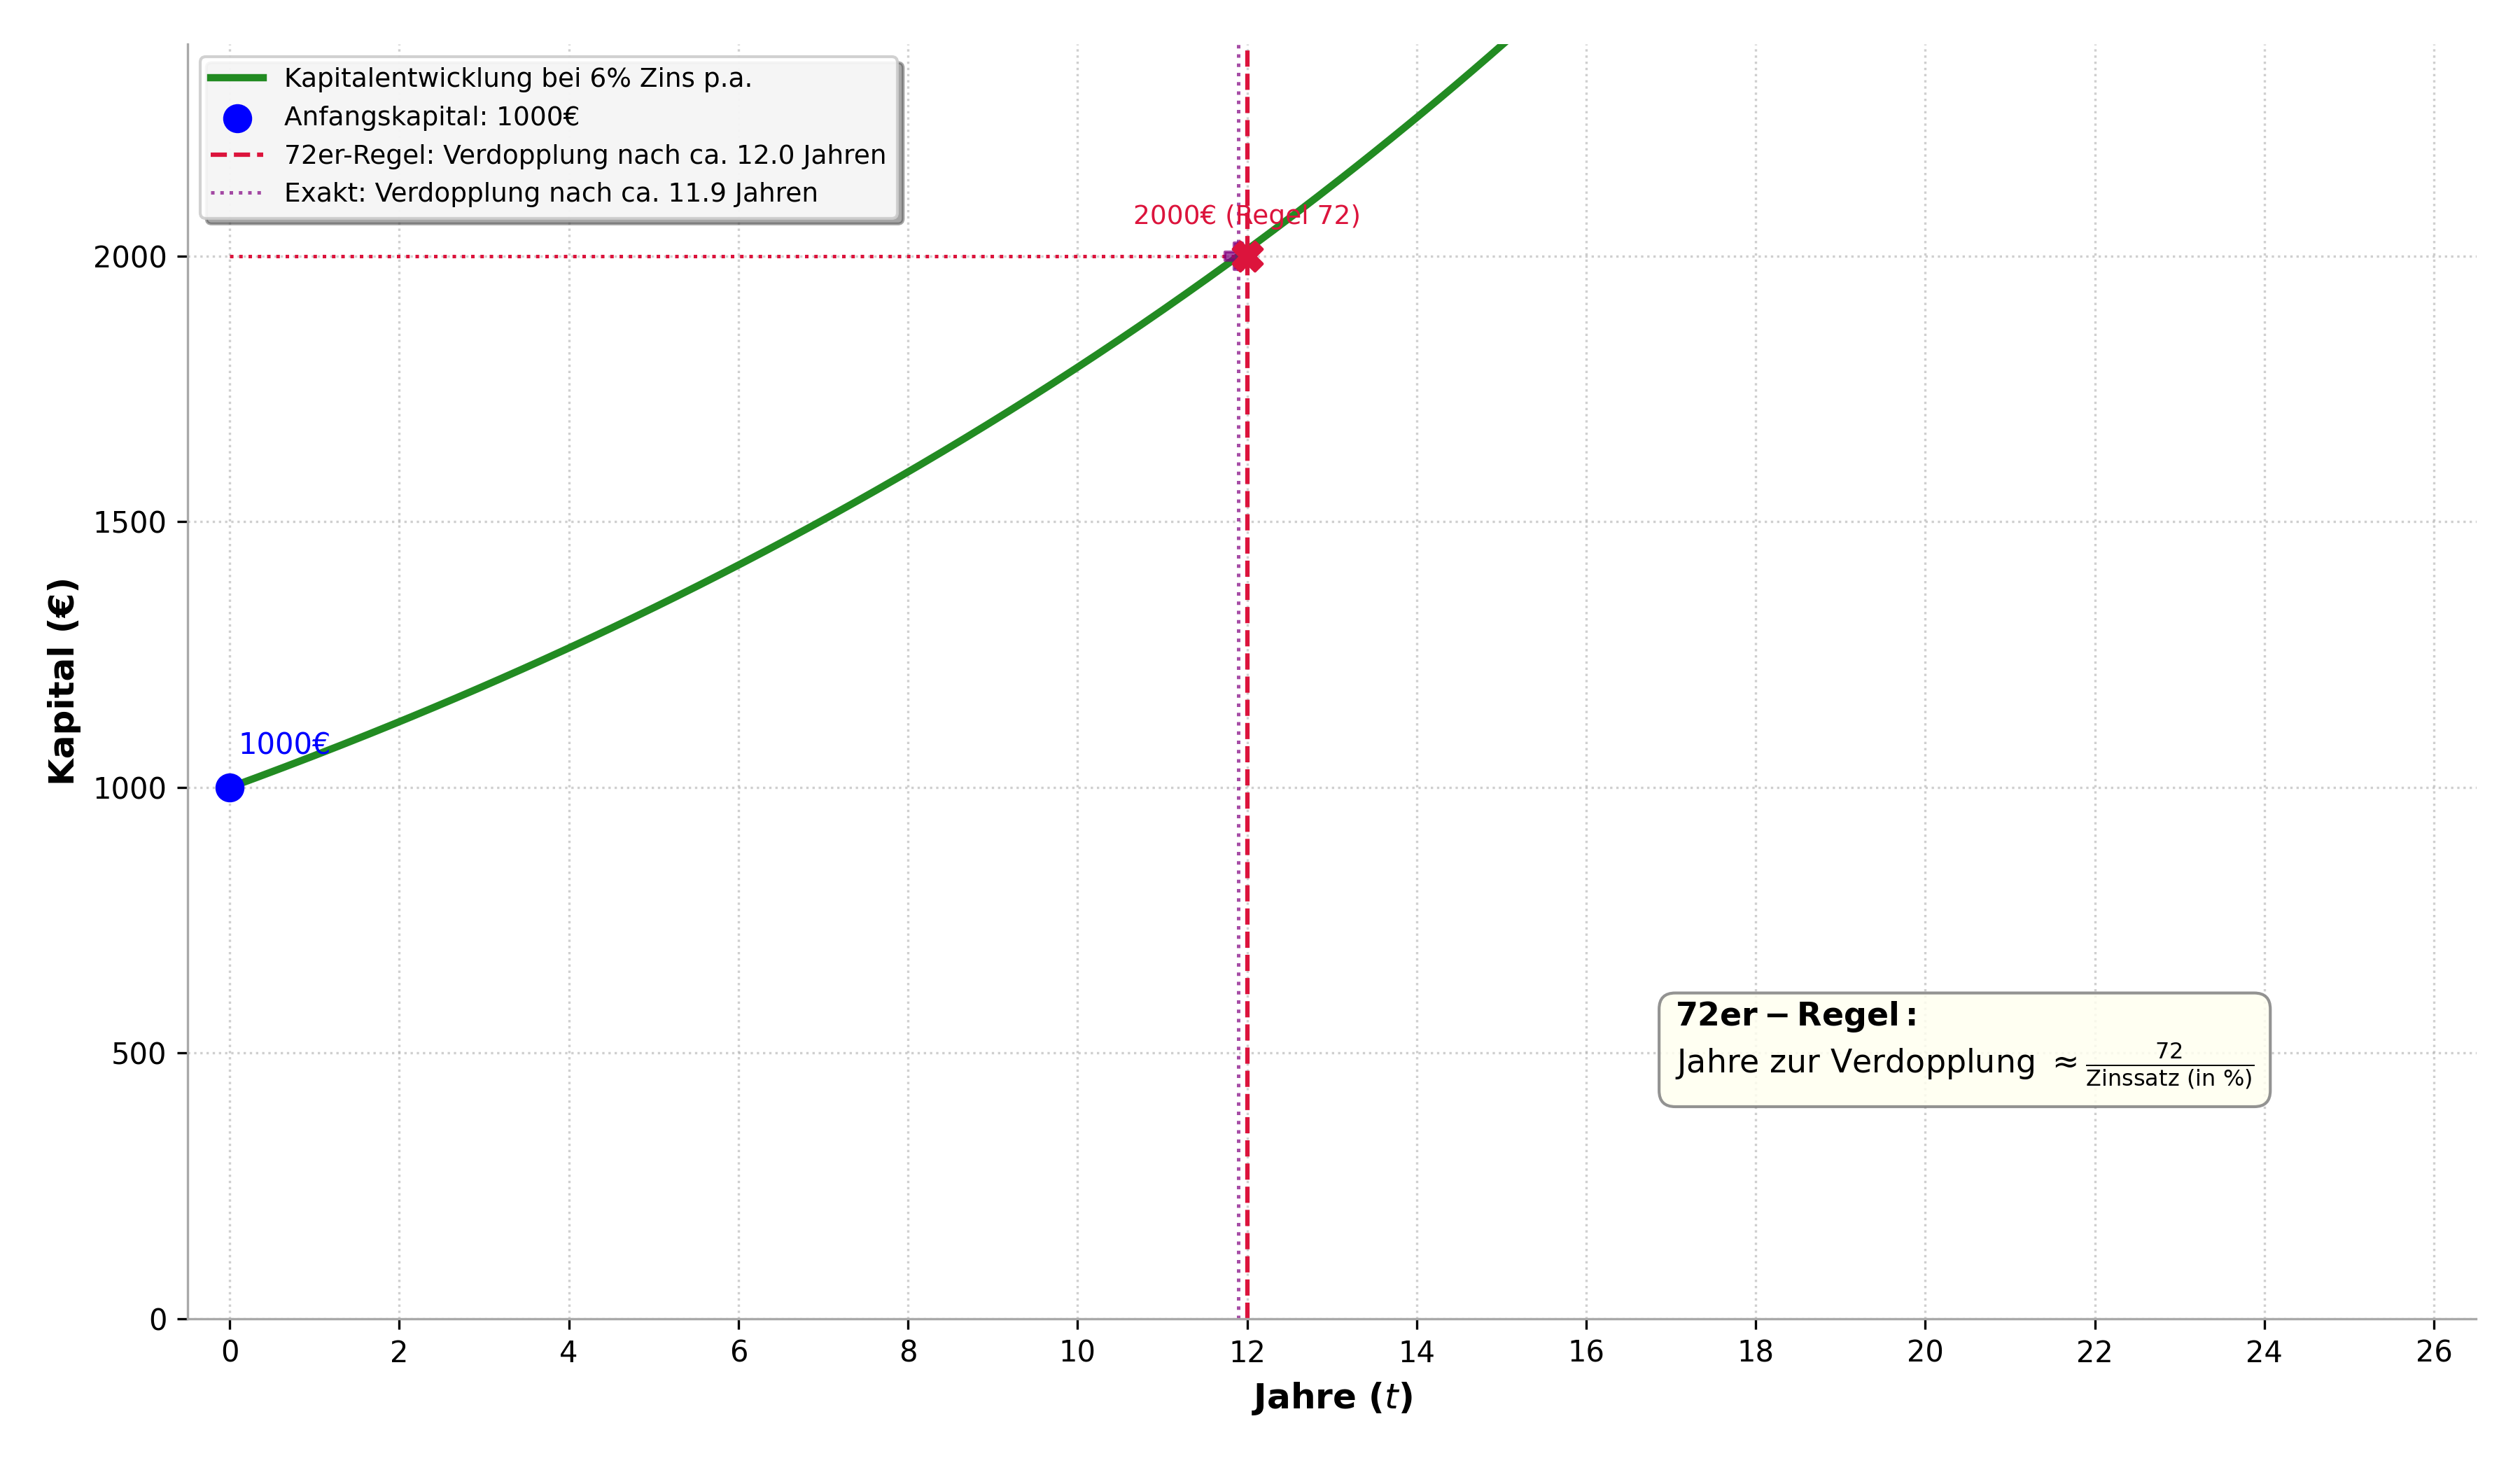
\includegraphics[width=0.5\textwidth]{grafiken/Regel_72_Zins.png}
    % Beschreibung für die Grafik 'Regel_72_Zins.png':
    % Die Grafik könnte ein Sparschwein zeigen, aus dem symbolisch Geld wächst
    % und sich verdoppelt. Daneben die Formel 'ca. 72 / Zinssatz (in %) = Jahre zur Verdopplung'.
    % Oder ein einfacher Graph exponentiellen Wachstums mit einer Markierung, 
    % wo sich der Anfangswert verdoppelt hat.
    \captionof{figure}{Die 72er-Regel: Eine Faustformel zur Verdopplungszeit.}
    \label{fig:regel_72_funfact}
\end{center}
\end{funfactbox}

\subsection{Die natürliche Exponentialfunktion $f(x) = e^x$ und die Eulersche Zahl $e$}
\label{subsec:natuerliche_exp_funktion}

Unter allen Exponentialfunktionen gibt es eine mit einer ganz besonderen Basis, die in der Mathematik eine herausragende Rolle spielt: die \textbf{natürliche Exponentialfunktion} $f(x) = e^x$. Die Basis dieser Funktion ist die \textbf{Eulersche Zahl $e$}.

\begin{merksatzumgebung}{Die Eulersche Zahl $e$}
Die Eulersche Zahl $e$ ist eine irrationale (nicht als Bruch ganzer Zahlen darstellbare) und transzendente Zahl mit dem ungefähren Wert:
\[ e \approx 2,718281828459... \]
Sie ist eine der wichtigsten Konstanten in der Mathematik, ähnlich wie $\pi$.
Eine Möglichkeit, $e$ zu definieren, ist über den Grenzwert (siehe Infobox im vorherigen Kapitel):
\[ e = \lim_{n \to \infty} \left(1 + \frac{1}{n}\right)^n \]
Diese Definition stammt aus der Zinseszinsrechnung bei kontinuierlicher Verzinsung.
\end{merksatzumgebung}

\begin{infoboxumgebung}{Warum ist $e$ so 'natürlich'?}
Die natürliche Exponentialfunktion $f(x)=e^x$ hat eine einzigartige und bemerkenswerte Eigenschaft, die sie so 'natürlich' und fundamental für die Differentialrechnung macht: \textbf{Sie ist ihre eigene Ableitung!}
\[ (e^x)' = e^x \]
Das bedeutet, die Steigung der Tangente an den Graphen von $f(x)=e^x$ an jeder Stelle $x$ ist genau gleich dem Funktionswert $e^x$ an dieser Stelle. An der Stelle $x=0$ ist $f(0)=e^0=1$, und die Steigung der Tangente ist ebenfalls $f'(0)=e^0=1$.
Diese Eigenschaft macht das Rechnen mit $e^x$ besonders elegant.
\end{infoboxumgebung}

\subsubsection{Graph und Eigenschaften von $f(x)=e^x$}

\begin{merksatzumgebung}{Eigenschaften der natürlichen Exponentialfunktion $f(x)=e^x$}
\begin{itemize}
    \item \textbf{Definitionsbereich:} $D_f = \mathbb{R}$ (man kann jede reelle Zahl für $x$ einsetzen).
    \item \textbf{Wertebereich:} $W_f = \mathbb{R}^+ = (0, \infty)$ (die Funktionswerte sind immer positiv und werden niemals Null oder negativ).
    \item \textbf{Nullstellen:} Die Funktion $f(x)=e^x$ hat \textbf{keine Nullstellen}, da $e^x > 0$ für alle $x \in \mathbb{R}$. Der Graph schneidet die x-Achse nie.
    \item \textbf{Schnittpunkt mit der y-Achse:} $f(0) = e^0 = 1$. Der Punkt ist $P_y(0|1)$.
    \item \textbf{Monotonie:} Da die Ableitung $f'(x)=e^x$ immer positiv ist ($e^x > 0$ für alle $x$), ist die Funktion $f(x)=e^x$ \textbf{streng monoton steigend} für alle $x \in \mathbb{R}$.
    \item \textbf{Krümmung:} Die zweite Ableitung ist $f''(x)=(e^x)'=e^x$. Da $f''(x)=e^x$ immer positiv ist, ist der Graph von $f(x)=e^x$ für alle $x \in \mathbb{R}$ \textbf{linksgekrümmt} (konvex).
    \item \textbf{Grenzwerte (Verhalten im Unendlichen):}
        \begin{itemize}
            \item $\lim_{x \to \infty} e^x = +\infty$ (für große positive $x$ werden die Werte beliebig groß).
            \item $\lim_{x \to -\infty} e^x = 0$ (für große negative $x$ nähern sich die Werte der Null an; die x-Achse ist eine \textbf{waagerechte Asymptote} für $x \to -\infty$).
        \end{itemize}
\end{itemize}
\end{merksatzumgebung}

\begin{center}
    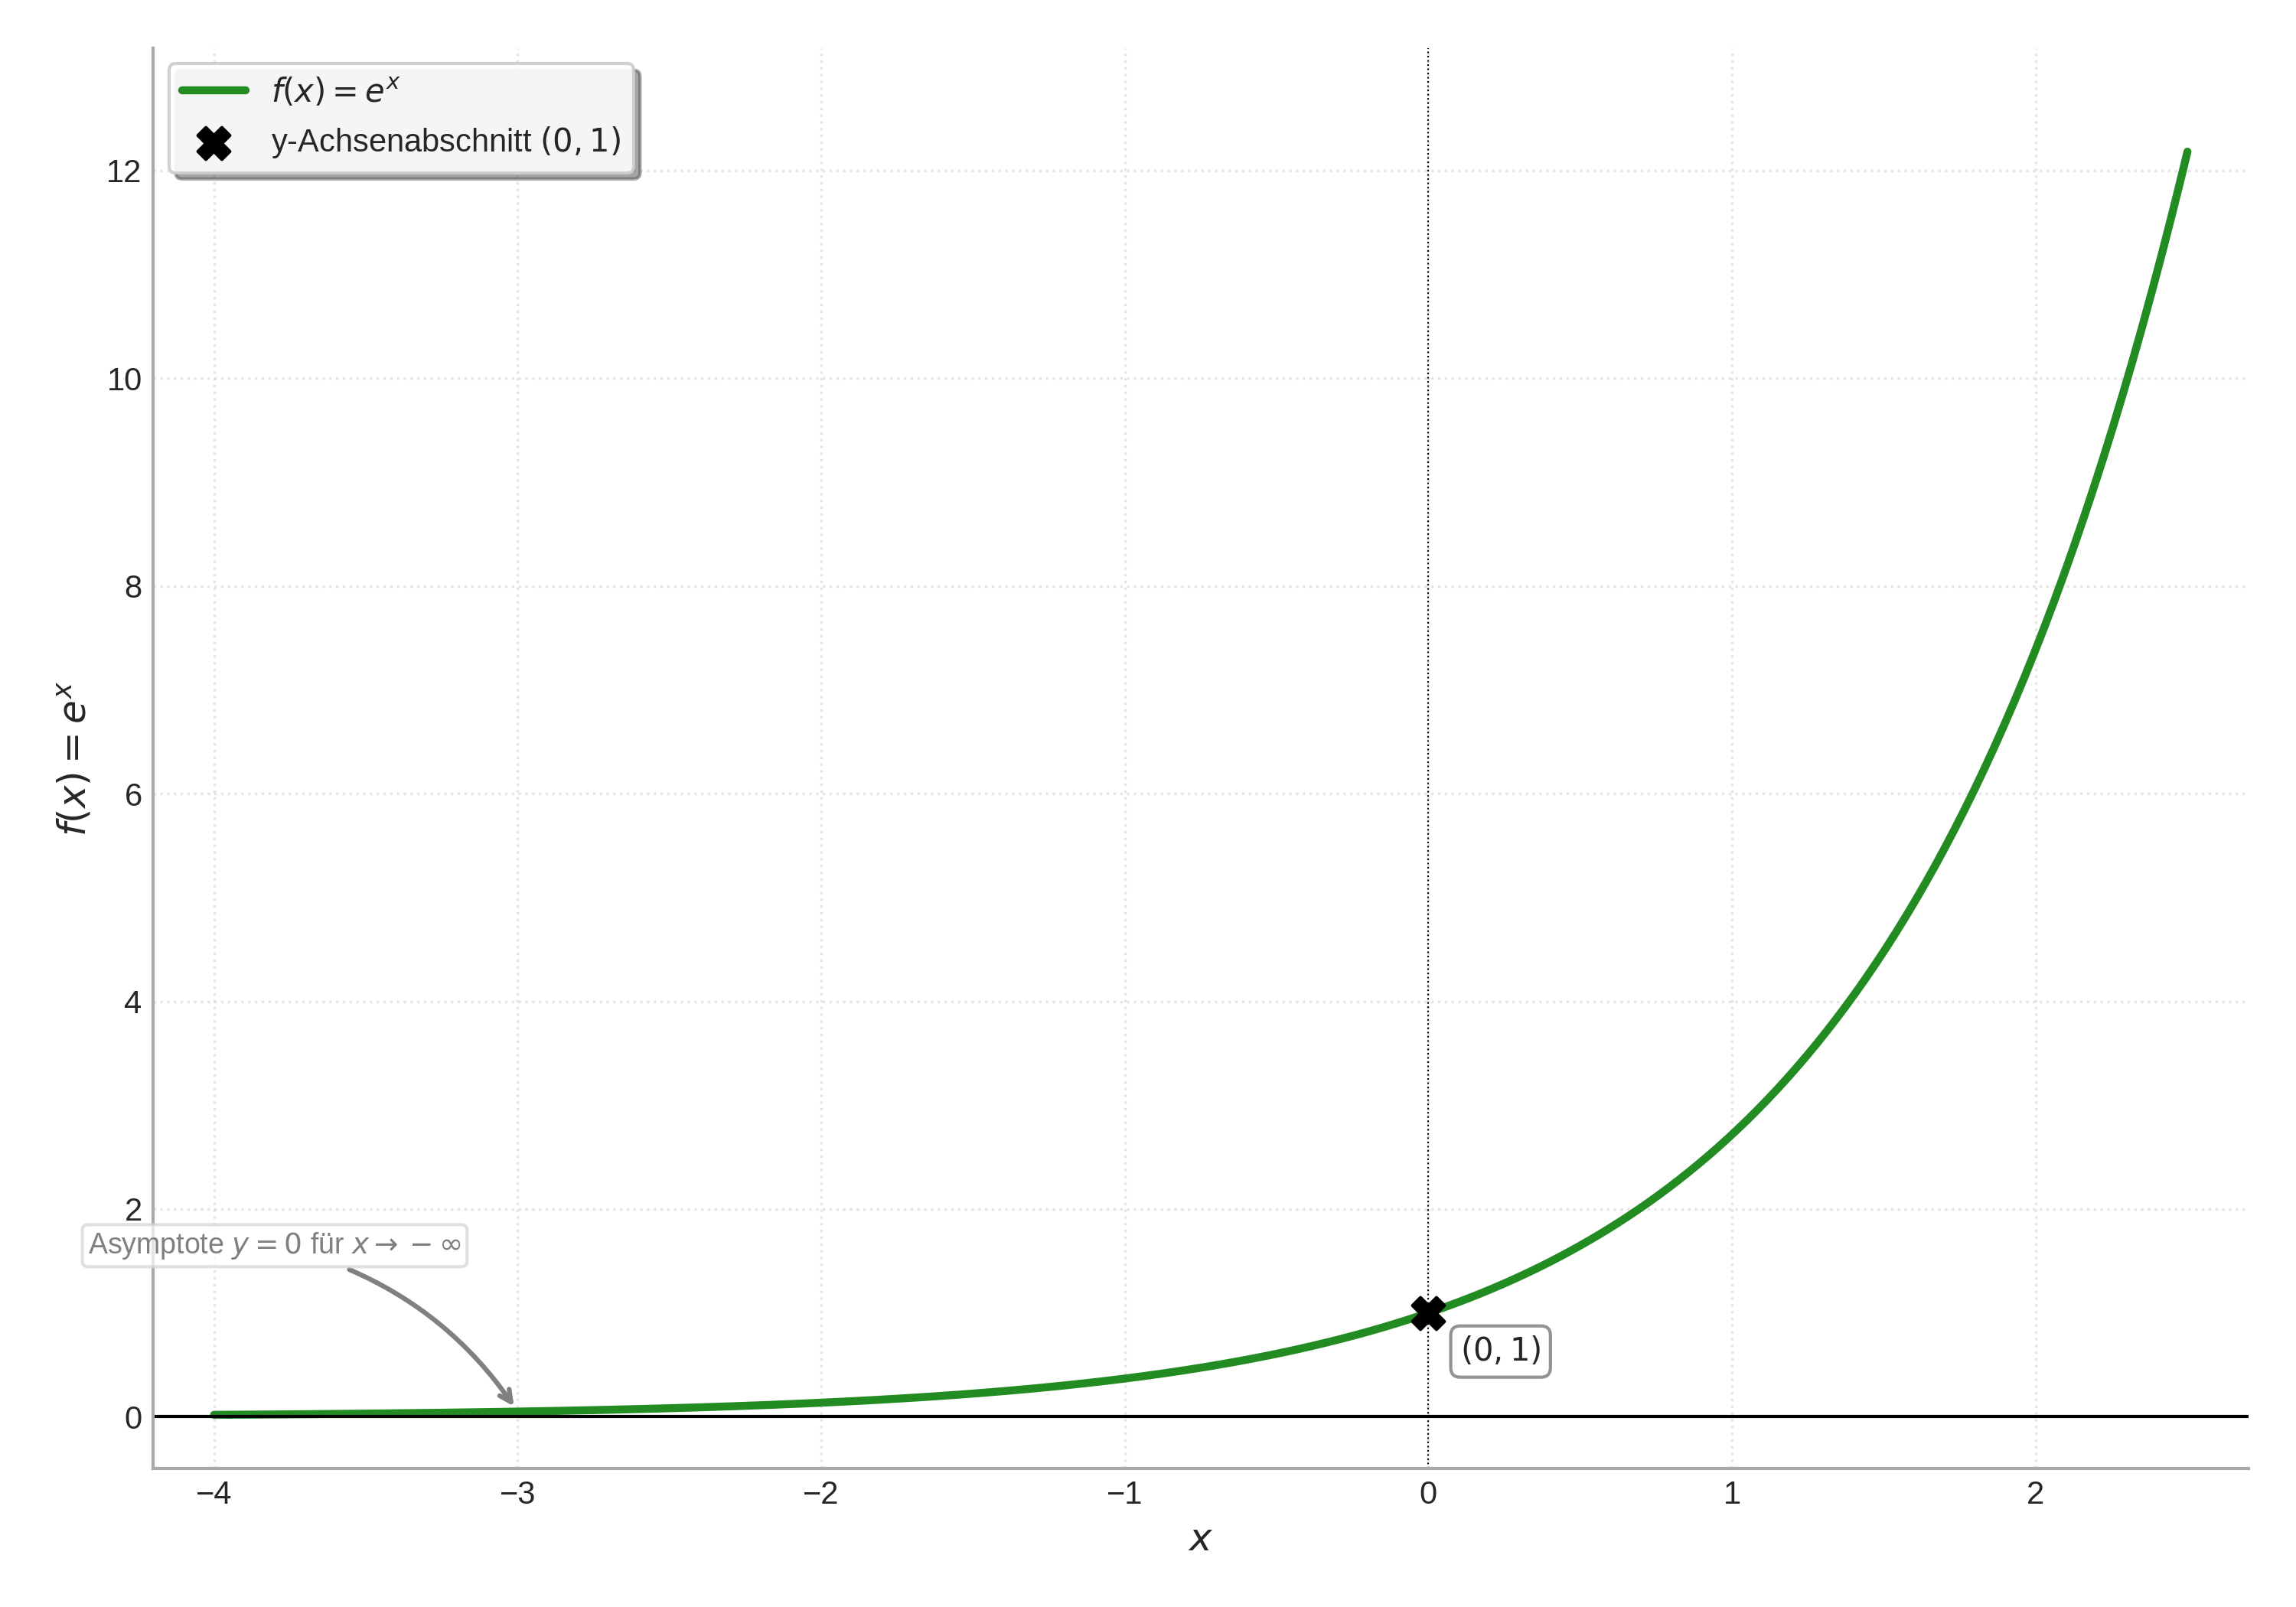
\includegraphics[width=0.8\textwidth]{grafiken/Exponentialfunktion_ex.png}
    \captionof{figure}{Graph der natürlichen Exponentialfunktion $f(x)=e^x$}
    \label{fig:exp_funktion_ex}
\end{center}

\subsubsection{Ableitung und Stammfunktion von $e^x$}

Wie bereits erwähnt, ist das Ableiten von $e^x$ besonders einfach.

\begin{merksatzumgebung}{Ableitung und Stammfunktion von $f(x)=e^x$}
\begin{itemize}
    \item \textbf{Ableitung:} Die Ableitung der natürlichen Exponentialfunktion $f(x)=e^x$ ist die Funktion selbst:
    \[ (e^x)' = e^x \]
    \item \textbf{Stammfunktion (unbestimmtes Integral):} Da die Ableitung von $e^x$ wieder $e^x$ ist, ist $e^x$ auch eine Stammfunktion von sich selbst. Die Menge aller Stammfunktionen ist:
    \[ \int e^x \,dx = e^x + C \]
    wobei $C$ die Integrationskonstante ist.
\end{itemize}
\end{merksatzumgebung}

\begin{beispielumgebung}{Ableiten und Integrieren von $e^x$}
\begin{enumerate}
    \item Leite $f(x) = 5e^x - 3x^2$ ab.
        $f'(x) = (5e^x)' - (3x^2)' = 5(e^x)' - 3(2x) = 5e^x - 6x$.
    \item Bestimme das unbestimmte Integral von $g(x) = 2e^x + 4x$.
        $\int (2e^x + 4x) \,dx = \int 2e^x \,dx + \int 4x \,dx$
        $= 2 \int e^x \,dx + 4 \int x^1 \,dx$
        $= 2e^x + 4 \cdot \frac{1}{2}x^2 + C = 2e^x + 2x^2 + C$.
\end{enumerate}
\end{beispielumgebung}

\begin{aufgabenumgebung}{Erste Übungen mit $e^x$}
\begin{enumerate}
    \item Bilde die erste und zweite Ableitung der folgenden Funktionen:
        \begin{itemize}
            \item $f_1(x) = 3e^x - x^3 + 2x - 7$
            \item $f_2(x) = -0.5e^x + \frac{1}{x}$ (Tipp: $\frac{1}{x} = x^{-1}$)
        \end{itemize}
    \item Bestimme die Menge aller Stammfunktionen:
        \begin{itemize}
            \item $g_1(x) = 4e^x + 6x^2 - 1$
            \item $g_2(x) = \frac{e^x}{2} - \sqrt{x}$ (Tipp: $\frac{e^x}{2} = \frac{1}{2}e^x$)
        \end{itemize}
    \item Berechne das bestimmte Integral $\int_0^1 e^x \,dx$. Was stellt dieser Wert geometrisch dar?
\end{enumerate}
\end{aufgabenumgebung}

\subsection{Allgemeinere Exponentialfunktionen und ihre Transformationen}
\label{subsec:allgemeine_exp_funktionen}

Die natürliche Exponentialfunktion $f(x)=e^x$ ist die Basis, aber oft begegnen uns Exponentialfunktionen in allgemeinerer Form, z.B. $f(x) = a \cdot e^{kx} + d$ oder $f(x) = a \cdot b^x$. Diese entstehen durch Transformationen (Streckung, Stauchung, Spiegelung, Verschiebung) der Grundfunktion $e^x$ oder einer anderen Basis $b$.

\subsubsection{Transformationen der natürlichen Exponentialfunktion: $f(x) = a \cdot e^{k(x-c)} + d$}

Ähnlich wie bei Polynomfunktionen können wir die Parameter interpretieren:
\begin{itemize}
    \item $a$: Streckung/Stauchung in y-Richtung. Wenn $a<0$, zusätzlich Spiegelung an der x-Achse.
    \item $k$: Streckung/Stauchung in x-Richtung. Wenn $k<0$, zusätzlich Spiegelung an der y-Achse. Beeinflusst die 'Schnelligkeit' des Wachstums/Zerfalls.
    \item $c$: Verschiebung in x-Richtung (um $c$ nach rechts, wenn $x-c$; um $c$ nach links, wenn $x+c$).
    \item $d$: Verschiebung in y-Richtung. Die Gerade $y=d$ wird zur neuen \textbf{waagerechten Asymptote}.
\end{itemize}

\textbf{Ableitung von $f(x) = e^{kx}$ (mit Kettenregel):}
Hier ist die äußere Funktion $g(u)=e^u$ mit $g'(u)=e^u$.
Die innere Funktion ist $h(x)=kx$ mit $h'(x)=k$.
Nach der Kettenregel: $(e^{kx})' = g'(h(x)) \cdot h'(x) = e^{kx} \cdot k = k e^{kx}$.

\begin{merksatzumgebung}{Ableitung und Stammfunktion von $e^{kx}$}
\begin{itemize}
    \item \textbf{Ableitung:} $(e^{kx})' = k \cdot e^{kx}$ (Kettenregel: 'äußere Ableitung $e^{kx}$ mal innere Ableitung $k$')
    \item \textbf{Stammfunktion:} $\int e^{kx} \,dx = \frac{1}{k} e^{kx} + C$ (für $k \neq 0$)
\end{itemize}
\end{merksatzumgebung}

\begin{beispielumgebung}{Ableiten und Integrieren von $a \cdot e^{kx}$}
\begin{enumerate}
    \item $f(x) = 3e^{2x}$. Hier ist $a=3, k=2$.
        $f'(x) = 3 \cdot (e^{2x})' = 3 \cdot (2e^{2x}) = 6e^{2x}$.
    \item $g(x) = -4e^{-0.5x} + 7$.
        $g'(x) = -4 \cdot (e^{-0.5x})' + (7)' = -4 \cdot (-0.5 e^{-0.5x}) + 0 = 2e^{-0.5x}$.
    \item $\int 5e^{3x} \,dx = 5 \int e^{3x} \,dx = 5 \cdot \frac{1}{3}e^{3x} + C = \frac{5}{3}e^{3x} + C$.
    \item $\int (e^{-x} + 2) \,dx = \int e^{-1x} \,dx + \int 2 \,dx = \frac{1}{-1}e^{-x} + 2x + C = -e^{-x} + 2x + C$.
\end{enumerate}
\end{beispielumgebung}

\begin{aufgabenumgebung}{Transformationen und Ableitungen/Stammfunktionen}
\begin{enumerate}
    \item Beschreibe, wie der Graph der Funktion $f(x) = 2e^{-0.5(x-1)} + 3$ aus dem Graphen der natürlichen Exponentialfunktion $y=e^x$ hervorgeht. Gib den Definitionsbereich, Wertebereich und die Gleichung der Asymptote an. Skizziere den Graphen.
    \item Bilde die erste Ableitung der folgenden Funktionen:
        \begin{itemize}
            \item $f_1(x) = 7e^{4x}$
            \item $f_2(x) = e^{-x} + 3x$
            \item $f_3(t) = A \cdot e^{-kt}$ ($A, k$ sind positive Konstanten; oft Modell für Zerfall)
        \end{itemize}
    \item Bestimme die Menge aller Stammfunktionen:
        \begin{itemize}
            \item $g_1(x) = 10e^{0.2x}$
            \item $g_2(x) = e^{-3x} - e^{2x}$
        \end{itemize}
\end{enumerate}
\end{aufgabenumgebung}

% Hier geht es dann weiter mit allgemeinen Basen b^x, Produkt/Quotient/Kette mit e-Funktionen, Kurvendiskussionen und Anwendungen.


% Vorheriger Inhalt des Kapitels bis zur aufgabenumgebung 'Transformationen und Ableitungen/Stammfunktionen'
% ... (siehe vorherige Canvas-Version) ...

\subsubsection{Die allgemeine Exponentialfunktion $f(x) = b^x$ und ihre Beziehung zu $e^x$}
\label{subsubsec:allgemeine_basis_b}

Neben der natürlichen Exponentialfunktion $f(x)=e^x$ gibt es natürlich auch Exponentialfunktionen zu jeder beliebigen positiven Basis $b$ (wobei $b \neq 1$), wie zum Beispiel $f(x)=2^x$, $f(x)=10^x$ oder $f(x)=(0.5)^x$.

\begin{merksatzumgebung}{Die allgemeine Exponentialfunktion $f(x)=b^x$}
Eine Funktion der Form
\[ f(x) = b^x \]
mit einer festen Basis $b > 0$ und $b \neq 1$ heißt allgemeine Exponentialfunktion zur Basis $b$.
\begin{itemize}
    \item Wenn $b > 1$: Die Funktion ist streng monoton steigend (Wachstum).
    \item Wenn $0 < b < 1$: Die Funktion ist streng monoton fallend (Zerfall).
\end{itemize}
Alle diese Funktionen gehen durch den Punkt $(0|1)$, denn $b^0=1$.
Ihre waagerechte Asymptote ist die x-Achse ($y=0$) für $x \to -\infty$ (wenn $b>1$) oder für $x \to \infty$ (wenn $0<b<1$).
\end{merksatzumgebung}

\begin{infoboxumgebung}{Warum reicht es oft, $e^x$ zu betrachten? Der Trick mit dem Logarithmus!}
Jede Exponentialfunktion $f(x)=b^x$ (mit $b>0$) lässt sich mit Hilfe des natürlichen Logarithmus ($\ln$) und der $e$-Funktion umschreiben. Es gilt nämlich:
\[ b = e^{\ln(b)} \]
(Da $e^x$ und $\ln(x)$ Umkehrfunktionen voneinander sind, heben sie sich sozusagen gegenseitig auf).
Damit können wir schreiben:
\[ b^x = (e^{\ln(b)})^x \]
Nach den Potenzgesetzen ($(a^m)^n = a^{m \cdot n}$) gilt:
\[ b^x = e^{\ln(b) \cdot x} = e^{x \ln(b)} \]
Der Term $\ln(b)$ ist dabei einfach eine Konstante für eine feste Basis $b$. Wenn wir also $k = \ln(b)$ setzen, haben wir die Form $e^{kx}$, die wir schon kennen!
Das bedeutet: \textbf{Jede Exponentialfunktion $b^x$ kann als natürliche Exponentialfunktion $e^{kx}$ mit $k=\ln(b)$ dargestellt werden.}
Deshalb ist die $e$-Funktion so fundamental: Verstehen wir sie und ihre Transformationen, verstehen wir im Grunde alle Exponentialfunktionen.

\textbf{Beispiele für die Umrechnung:}
\begin{itemize}
    \item $2^x = e^{\ln(2) \cdot x} \approx e^{0.693x}$
    \item $10^x = e^{\ln(10) \cdot x} \approx e^{2.303x}$
    \item $(0.5)^x = e^{\ln(0.5) \cdot x} \approx e^{-0.693x}$ (Hier ist $\ln(0.5) = \ln(1/2) = \ln(1)-\ln(2) = 0-\ln(2) = -\ln(2) < 0$, was zum erwarteten Zerfall führt).
\end{itemize}
\end{infoboxumgebung}

\textbf{Ableitung von $f(x) = b^x$:}
Mit dem Trick $b^x = e^{x \ln(b)}$ und der Kettenregel können wir $b^x$ leicht ableiten:
Sei $f(x) = b^x = e^{x \ln(b)}$.
Die äußere Funktion ist $g(u)=e^u \implies g'(u)=e^u$.
Die innere Funktion ist $h(x)=x \ln(b) \implies h'(x)=\ln(b)$ (da $\ln(b)$ eine Konstante ist und die Ableitung von $kx$ gleich $k$ ist).
Also nach der Kettenregel:
$(b^x)' = (e^{x \ln(b)})' = e^{x \ln(b)} \cdot \ln(b) = b^x \cdot \ln(b)$.

\begin{merksatzumgebung}{Ableitung und Stammfunktion von $f(x)=b^x$}
\begin{itemize}
    \item \textbf{Ableitung:} Die Ableitung der allgemeinen Exponentialfunktion $f(x)=b^x$ ist:
    \[ (b^x)' = b^x \cdot \ln(b) \]
    (Beachte: Für $b=e$ ist $\ln(e)=1$, also $(e^x)' = e^x \cdot 1 = e^x$, was wir schon wussten!)
    \item \textbf{Stammfunktion:} Die Menge aller Stammfunktionen von $f(x)=b^x$ ist:
    \[ \int b^x \,dx = \frac{1}{\ln(b)} b^x + C \quad (\text{für } b>0, b\neq 1) \]
    (Probe: $(\frac{1}{\ln(b)} b^x)' = \frac{1}{\ln(b)} (b^x \cdot \ln(b)) = b^x$. Passt!)
\end{itemize}
\end{merksatzumgebung}

\begin{beispielumgebung}{Ableiten und Integrieren von $b^x$}
\begin{enumerate}
    \item $f(x) = 2^x$.
        $f'(x) = 2^x \cdot \ln(2)$.
    \item $g(x) = 5 \cdot 10^x$.
        $g'(x) = 5 \cdot (10^x \cdot \ln(10)) = 5 \ln(10) \cdot 10^x$.
    \item $\int 3^x \,dx = \frac{1}{\ln(3)} 3^x + C$.
\end{enumerate}
\end{beispielumgebung}

\begin{aufgabenumgebung}{Umgang mit allgemeinen Exponentialfunktionen}
\begin{enumerate}
    \item Schreibe die folgenden Funktionen mit der Basis $e$ (d.h. in der Form $a \cdot e^{kx}$):
        \begin{itemize}
            \item $f_1(x) = 3^x$
            \item $f_2(x) = 10 \cdot (0.8)^x$
        \end{itemize}
    \item Bilde die erste Ableitung der folgenden Funktionen:
        \begin{itemize}
            \item $g_1(x) = 4^x + x^4$
            \item $g_2(x) = 7 \cdot (1.5)^x - e^x$
            \item $g_3(t) = P_0 \cdot a^t$ ($P_0$ und $a$ sind positive Konstanten. Dies ist ein typisches Modell für exponentielles Wachstum oder Zerfall, je nachdem ob $a>1$ oder $0<a<1$.)
        \end{itemize}
    \item Bestimme die Menge aller Stammfunktionen:
        \begin{itemize}
            \item $h_1(x) = 5^x$
            \item $h_2(x) = 3 \cdot (0.2)^x + e^{2x}$
        \end{itemize}
    \item \textbf{Vergleich $2^x$ und $e^x$:}
        \begin{itemize}
            \item Skizziere die Graphen von $f(x)=2^x$ und $g(x)=e^x$ in ein gemeinsames Koordinatensystem (z.B. für $x \in [-2, 3]$). Nutze dazu eine Wertetabelle.
            \item Vergleiche die Steigungen der beiden Funktionen an der Stelle $x=0$. Welche Funktion wächst dort schneller?
            \item Berechne $(2^x)'$ und $(e^x)'$.
        \end{itemize}
\end{enumerate}
\end{aufgabenumgebung}

\begin{fehlerboxumgebung}{Ableiten von $e^{g(x)}$ und $b^x$}
Beim Ableiten von Exponentialfunktionen schleichen sich leicht Fehler ein. Achte besonders auf:
\begin{itemize}
    \item \textbf{Innere Ableitung bei $e^{g(x)}$ vergessen:} Die häufigste Fehlerquelle! Bei Funktionen wie $f(x) = e^{kx}$ oder allgemeiner $f(x) = e^{g(x)}$ musst du immer die Kettenregel anwenden: $(e^{g(x)})' = e^{g(x)} \cdot g'(x)$. Die Ableitung des Exponenten (innere Ableitung $g'(x)$) darf nicht fehlen!
    \textit{Beispiel Falsch:} $(e^{3x})' = e^{3x}$. \textit{Richtig:} $(e^{3x})' = e^{3x} \cdot 3 = 3e^{3x}$.
    \item \textbf{Faktor $\ln(b)$ bei $(b^x)'$ vergessen:} Die Ableitung von $f(x)=b^x$ ist $f'(x) = b^x \cdot \ln(b)$. Der Faktor $\ln(b)$ ist entscheidend (außer für $b=e$, da $\ln(e)=1$).
    \textit{Beispiel Falsch:} $(2^x)' = 2^x$. \textit{Richtig:} $(2^x)' = 2^x \cdot \ln(2)$.
    \item \textbf{Potenzregel falsch auf Basis $e$ oder $b$ angewendet:} Die Regel $(x^n)' = nx^{n-1}$ gilt, wenn die \textit{Basis} die Variable ist und der \textit{Exponent} eine Konstante. Bei $e^x$ oder $b^x$ ist die Basis eine Konstante und der Exponent die Variable.
    \textit{Beispiel Falsch:} $(e^x)' = xe^{x-1}$. \textit{Richtig:} $(e^x)' = e^x$.
\end{itemize}
Präge dir diese Unterschiede gut ein, um Fehler zu vermeiden!
\end{fehlerboxumgebung}

\begin{tippumgebung}{Taschenrechner für $\ln(b)$}
Den Wert von $\ln(b)$ (natürlicher Logarithmus von $b$) findest du auf deinem Taschenrechner (oft als 'ln'-Taste). Für viele theoretische Überlegungen und Ableitungen lässt man $\ln(b)$ aber einfach als exakten Ausdruck stehen.
\end{tippumgebung}

% Vorheriger Inhalt des Kapitels bis zur Tippumgebung 'Taschenrechner für ln(b)'
% ... (siehe vorherige Canvas-Version) ...

Die Fähigkeit, zwischen $b^x$ und $e^{kx}$ wechseln zu können, ist sehr nützlich, da viele Formeln und Regeln in der Analysis primär für die Basis $e$ formuliert sind.

\subsubsection{Anwendung der Ableitungsregeln auf Funktionen mit $e^x$}
\label{subsubsec:ableitungsregeln_ex}

Jetzt, da wir die Grundfunktionen $e^x$ und $e^{kx}$ sowie deren Ableitungen und Stammfunktionen kennen, wollen wir sehen, wie wir Funktionen ableiten, bei denen diese mit Polynomen durch Produkt, Quotient oder Verkettung verbunden sind. Hier kommen unsere bekannten Ableitungsregeln voll zum Einsatz!

\textbf{Produktregel mit $e^x$:}
Erinnerung: $(u \cdot v)' = u'v + uv'$.

\begin{beispielumgebung}{Produktregel mit $e^x$}
Leite $f(x) = x^2 \cdot e^x$ ab.
\begin{itemize}
    \item $u(x) = x^2 \implies u'(x) = 2x$
    \item $v(x) = e^x \implies v'(x) = e^x$
\end{itemize}
$f'(x) = (2x) \cdot e^x + x^2 \cdot e^x$
Hier kann man $e^x$ ausklammern:
$f'(x) = e^x (2x + x^2) = e^x (x^2 + 2x)$.
\end{beispielumgebung}

\begin{aufgabenumgebung}{Produktregel mit $e^x$ üben}
Bilde die erste Ableitung der folgenden Funktionen und vereinfache so weit wie möglich:
\begin{enumerate}
    \item $f_1(x) = (3x-1)e^x$
    \item $f_2(x) = (x^2+2x-5)e^x$
    \item $f_3(t) = t \cdot e^{2t}$ (Hier ist die Kettenregel für $e^{2t}$ zusätzlich nötig!)
\end{enumerate}
\end{aufgabenumgebung}

\textbf{Quotientenregel mit $e^x$:}
Erinnerung: $(\frac{u}{v})' = \frac{u'v - uv'}{v^2}$.

\begin{beispielumgebung}{Quotientenregel mit $e^x$}
Leite $f(x) = \frac{e^x}{x^2+1}$ ab. (Definitionsbereich $D_f = \mathbb{R}$)
\begin{itemize}
    \item $u(x) = e^x \implies u'(x) = e^x$
    \item $v(x) = x^2+1 \implies v'(x) = 2x$
\end{itemize}
$f'(x) = \frac{e^x \cdot (x^2+1) - e^x \cdot 2x}{(x^2+1)^2}$
Auch hier kann man $e^x$ im Zähler ausklammern:
$f'(x) = \frac{e^x (x^2+1 - 2x)}{(x^2+1)^2} = \frac{e^x (x^2-2x+1)}{(x^2+1)^2} = \frac{e^x (x-1)^2}{(x^2+1)^2}$.
\end{beispielumgebung}

\begin{aufgabenumgebung}{Quotientenregel mit $e^x$ üben}
Bilde die erste Ableitung der folgenden Funktionen und vereinfache so weit wie möglich. Gib auch den Definitionsbereich an.
\begin{enumerate}
    \item $f_1(x) = \frac{x+2}{e^x}$
    \item $f_2(x) = \frac{e^{3x}}{2x-1}$ (Kettenregel für $e^{3x}$ nötig!)
\end{enumerate}
\end{aufgabenumgebung}

\textbf{Kettenregel mit $e^x$ (Vertiefung):}
Erinnerung: $(g(h(x)))' = g'(h(x)) \cdot h'(x)$.
Die Exponentialfunktion tritt sehr oft als äußere Funktion auf, wobei der Exponent die innere Funktion ist.

\begin{beispielumgebung}{Kettenregel mit $e^x$ vertieft}
Leite $f(x) = e^{x^2-3x}$ ab.
\begin{itemize}
    \item Äußere Funktion: $g(u) = e^u \implies g'(u) = e^u$.
    \item Innere Funktion: $h(x) = x^2-3x \implies h'(x) = 2x-3$.
\end{itemize}
$f'(x) = g'(h(x)) \cdot h'(x) = e^{x^2-3x} \cdot (2x-3) = (2x-3)e^{x^2-3x}$.
\end{beispielumgebung}

\begin{aufgabenumgebung}{Kettenregel mit $e^x$ weiter üben}
Bilde die erste Ableitung:
\begin{enumerate}
    \item $f_1(x) = e^{-x^2}$
    \item $f_2(x) = 5e^{2x^3-4x+1}$
    \item $f_3(x) = (e^x+1)^3$ (Hier ist $e^x+1$ die innere Funktion und $(\dots)^3$ die äußere.)
\end{enumerate}
\end{aufgabenumgebung}



\begin{aufgabenumgebung}{Kombinierte Anwendung: Produkt- und Kettenregel bei e-Funktionen}
Bilde die erste Ableitung der folgenden Funktionen. Vereinfache das Ergebnis so weit wie möglich, indem du z.B. gemeinsame Faktoren (insbesondere den $e$-Term) ausklammerst.
\begin{enumerate}
    \item $f(x) = (2x^2 - 3x + 1) \cdot e^{x^2 - 4}$
        \begin{tippumgebung}{Struktur erkennen}
        Diese Funktion ist ein Produkt $u(x) \cdot v(x)$. Für die Ableitung des Faktors $v(x)=e^{x^2-4}$ benötigst du die Kettenregel.
        \end{tippumgebung}
    \item $g(x) = (x+1)^2 \cdot e^{-2x}$
        \begin{tippumgebung}{Zweimal Kettenregel?}
        Auch dies ist ein Produkt. Ein Faktor ist $(x+1)^2$, dessen Ableitung die Kettenregel (oder Ausmultiplizieren) erfordert. Der andere Faktor $e^{-2x}$ benötigt ebenfalls die Kettenregel.
        \end{tippumgebung}
\end{enumerate}
\end{aufgabenumgebung}


\subsection{Kurvendiskussion von Funktionen mit $e^x$}
\label{subsec:kurvendiskussion_ex}

Jetzt, da wir wissen, wie man Funktionen mit $e^x$ ableitet, können wir auch für sie eine vollständige Kurvendiskussion durchführen. Ein wichtiger Punkt bei der Nullstellensuche ist die Eigenschaft der $e$-Funktion.

\begin{infoboxumgebung}{Nullstellen von Produkten mit $e^x$ – Eine wichtige Erkenntnis}
Wir wissen, dass $e^x > 0$ für alle reellen Zahlen $x$ gilt. Die natürliche Exponentialfunktion hat also \textbf{keine Nullstellen}.
Das hat eine wichtige Konsequenz für Produkte der Form $f(x) = \text{Polynom}(x) \cdot e^x$ oder allgemeiner $f(x) = h(x) \cdot e^{g(x)}$:
Nach dem Satz vom Nullprodukt ist ein Produkt genau dann Null, wenn mindestens einer seiner Faktoren Null ist. Da $e^x$ (oder $e^{g(x)}$) niemals Null werden kann, hängen die Nullstellen von $f(x)$ \textbf{ausschließlich von den Nullstellen des Faktors $\text{Polynom}(x)$ (bzw. $h(x)$) ab}.

Um die Nullstellen von $f(x) = \text{Polynom}(x) \cdot e^x$ zu finden, reicht es also, die Gleichung $\text{Polynom}(x) = 0$ zu lösen.
\end{infoboxumgebung}

\begin{beispielumgebung}[Kurvendiskussion einer e-Funktion mit Polynom]{Untersuchung von $f(x) = (x-1)e^x$}
\begin{enumerate}
    \item \textbf{Definitionsbereich:} $D_f = \mathbb{R}$ (sowohl $x-1$ als auch $e^x$ sind für alle $x$ definiert).
    \item \textbf{Symmetrie:}
        $f(-x) = (-x-1)e^{-x} = -(x+1)e^{-x}$.
        Keine einfache Symmetrie zum Koordinatensystem erkennbar.
    \item \textbf{Verhalten im Unendlichen:}
        \begin{itemize}
            \item Für $x \to \infty$: $(x-1) \to \infty$ und $e^x \to \infty$. Also $\lim_{x \to \infty} f(x) = \infty \cdot \infty = +\infty$.
            \item Für $x \to -\infty$: $(x-1) \to -\infty$. Aber $e^x \to 0$. Hier haben wir einen Konflikt '$-\infty \cdot 0$'. Es ist bekannt, dass die $e$-Funktion 'stärker' gegen Null geht als jedes Polynom gegen Unendlich. Man kann auch schreiben $f(x) = \frac{x-1}{e^{-x}}$. Für $x \to -\infty$ geht der Zähler gegen $-\infty$ und der Nenner $e^{-x}$ gegen $e^{\infty} = \infty$. Auch hier ist es nicht sofort klar.
            Ein wichtiger Grenzwert ist $\lim_{x \to -\infty} x^n e^x = 0$ für jedes $n \in \mathbb{N}$.
            Daher: $\lim_{x \to -\infty} (x-1)e^x = 0$. Die x-Achse ($y=0$) ist eine waagerechte Asymptote für $x \to -\infty$.
        \end{itemize}
    \item \textbf{y-Achsenabschnitt:} $f(0) = (0-1)e^0 = (-1) \cdot 1 = -1$. Also $P_y(0|-1)$.
    \item \textbf{Nullstellen:} $f(x)=0 \implies (x-1)e^x = 0$.
        Da $e^x \neq 0$ für alle $x$, muss $x-1=0$ sein.
        Also $x_N = 1$. Einzige Nullstelle bei $N(1|0)$.
    \item \textbf{Erste Ableitung $f'(x)$:} Mit Produktregel $u(x)=x-1, u'(x)=1, v(x)=e^x, v'(x)=e^x$.
        $f'(x) = 1 \cdot e^x + (x-1) \cdot e^x = e^x (1 + x - 1) = xe^x$.
    \item \textbf{Extremstellen:} $f'(x)=0 \implies xe^x = 0$.
        Da $e^x \neq 0$, muss $x=0$ sein. Potentielle Extremstelle bei $x_E=0$.
    \item \textbf{Zweite Ableitung $f''(x)$:} Mit Produktregel für $f'(x)=xe^x$: $u(x)=x, u'(x)=1, v(x)=e^x, v'(x)=e^x$.
        $f''(x) = 1 \cdot e^x + x \cdot e^x = e^x(1+x) = (x+1)e^x$.
    \item \textbf{Art der Extremstelle bei $x_E=0$ mit $f''$ prüfen:}
        $f''(0) = (0+1)e^0 = 1 \cdot 1 = 1$.
        Da $f'(0)=0$ und $f''(0)=1 > 0 \implies$ Lokaler Tiefpunkt bei $x_E=0$.
        $y_T = f(0) = -1$. Tiefpunkt $T(0|-1)$. (Das ist auch unser y-Achsenabschnitt).
    \item \textbf{Monotonie:} Nullstelle von $f'(x)=xe^x$ ist $x=0$.
        \begin{itemize}
            \item $x < 0$ (z.B. $x=-1$): $f'(-1) = (-1)e^{-1} = -1/e < 0 \implies$ fallend.
            \item $x > 0$ (z.B. $x=1$): $f'(1) = (1)e^{1} = e > 0 \implies$ steigend.
        \end{itemize}
        Fallend für $x \in (-\infty, 0]$, steigend für $x \in [0, \infty)$.
    \item \textbf{Wendepunkte:} $f''(x_W)=0 \implies (x_W+1)e^{x_W} = 0$.
        Da $e^{x_W} \neq 0$, muss $x_W+1=0 \implies x_W = -1$.
        Dritte Ableitung $f'''(x)$: Produktregel für $f''(x)=(x+1)e^x$. $u(x)=x+1, u'(x)=1, v(x)=e^x, v'(x)=e^x$.
        $f'''(x) = 1 \cdot e^x + (x+1)e^x = e^x(1+x+1) = (x+2)e^x$.
        $f'''(-1) = (-1+2)e^{-1} = 1 \cdot e^{-1} = 1/e \neq 0$.
        Also Wendepunkt bei $x_W=-1$.
        $y_W = f(-1) = (-1-1)e^{-1} = -2e^{-1} = -2/e \approx -0.736$.
        Wendepunkt $W(-1|-2/e)$.
    \item \textbf{Krümmungsverhalten:} Nullstelle von $f''(x)=(x+1)e^x$ ist $x=-1$.
        \begin{itemize}
            \item $x < -1$ (z.B. $x=-2$): $f''(-2) = (-2+1)e^{-2} = -e^{-2} < 0 \implies$ rechtsgekrümmt.
            \item $x > -1$ (z.B. $x=0$): $f''(0) = (0+1)e^{0} = 1 > 0 \implies$ linksgekrümmt.
        \end{itemize}
    \item \textbf{Skizze:}
        \begin{center}
            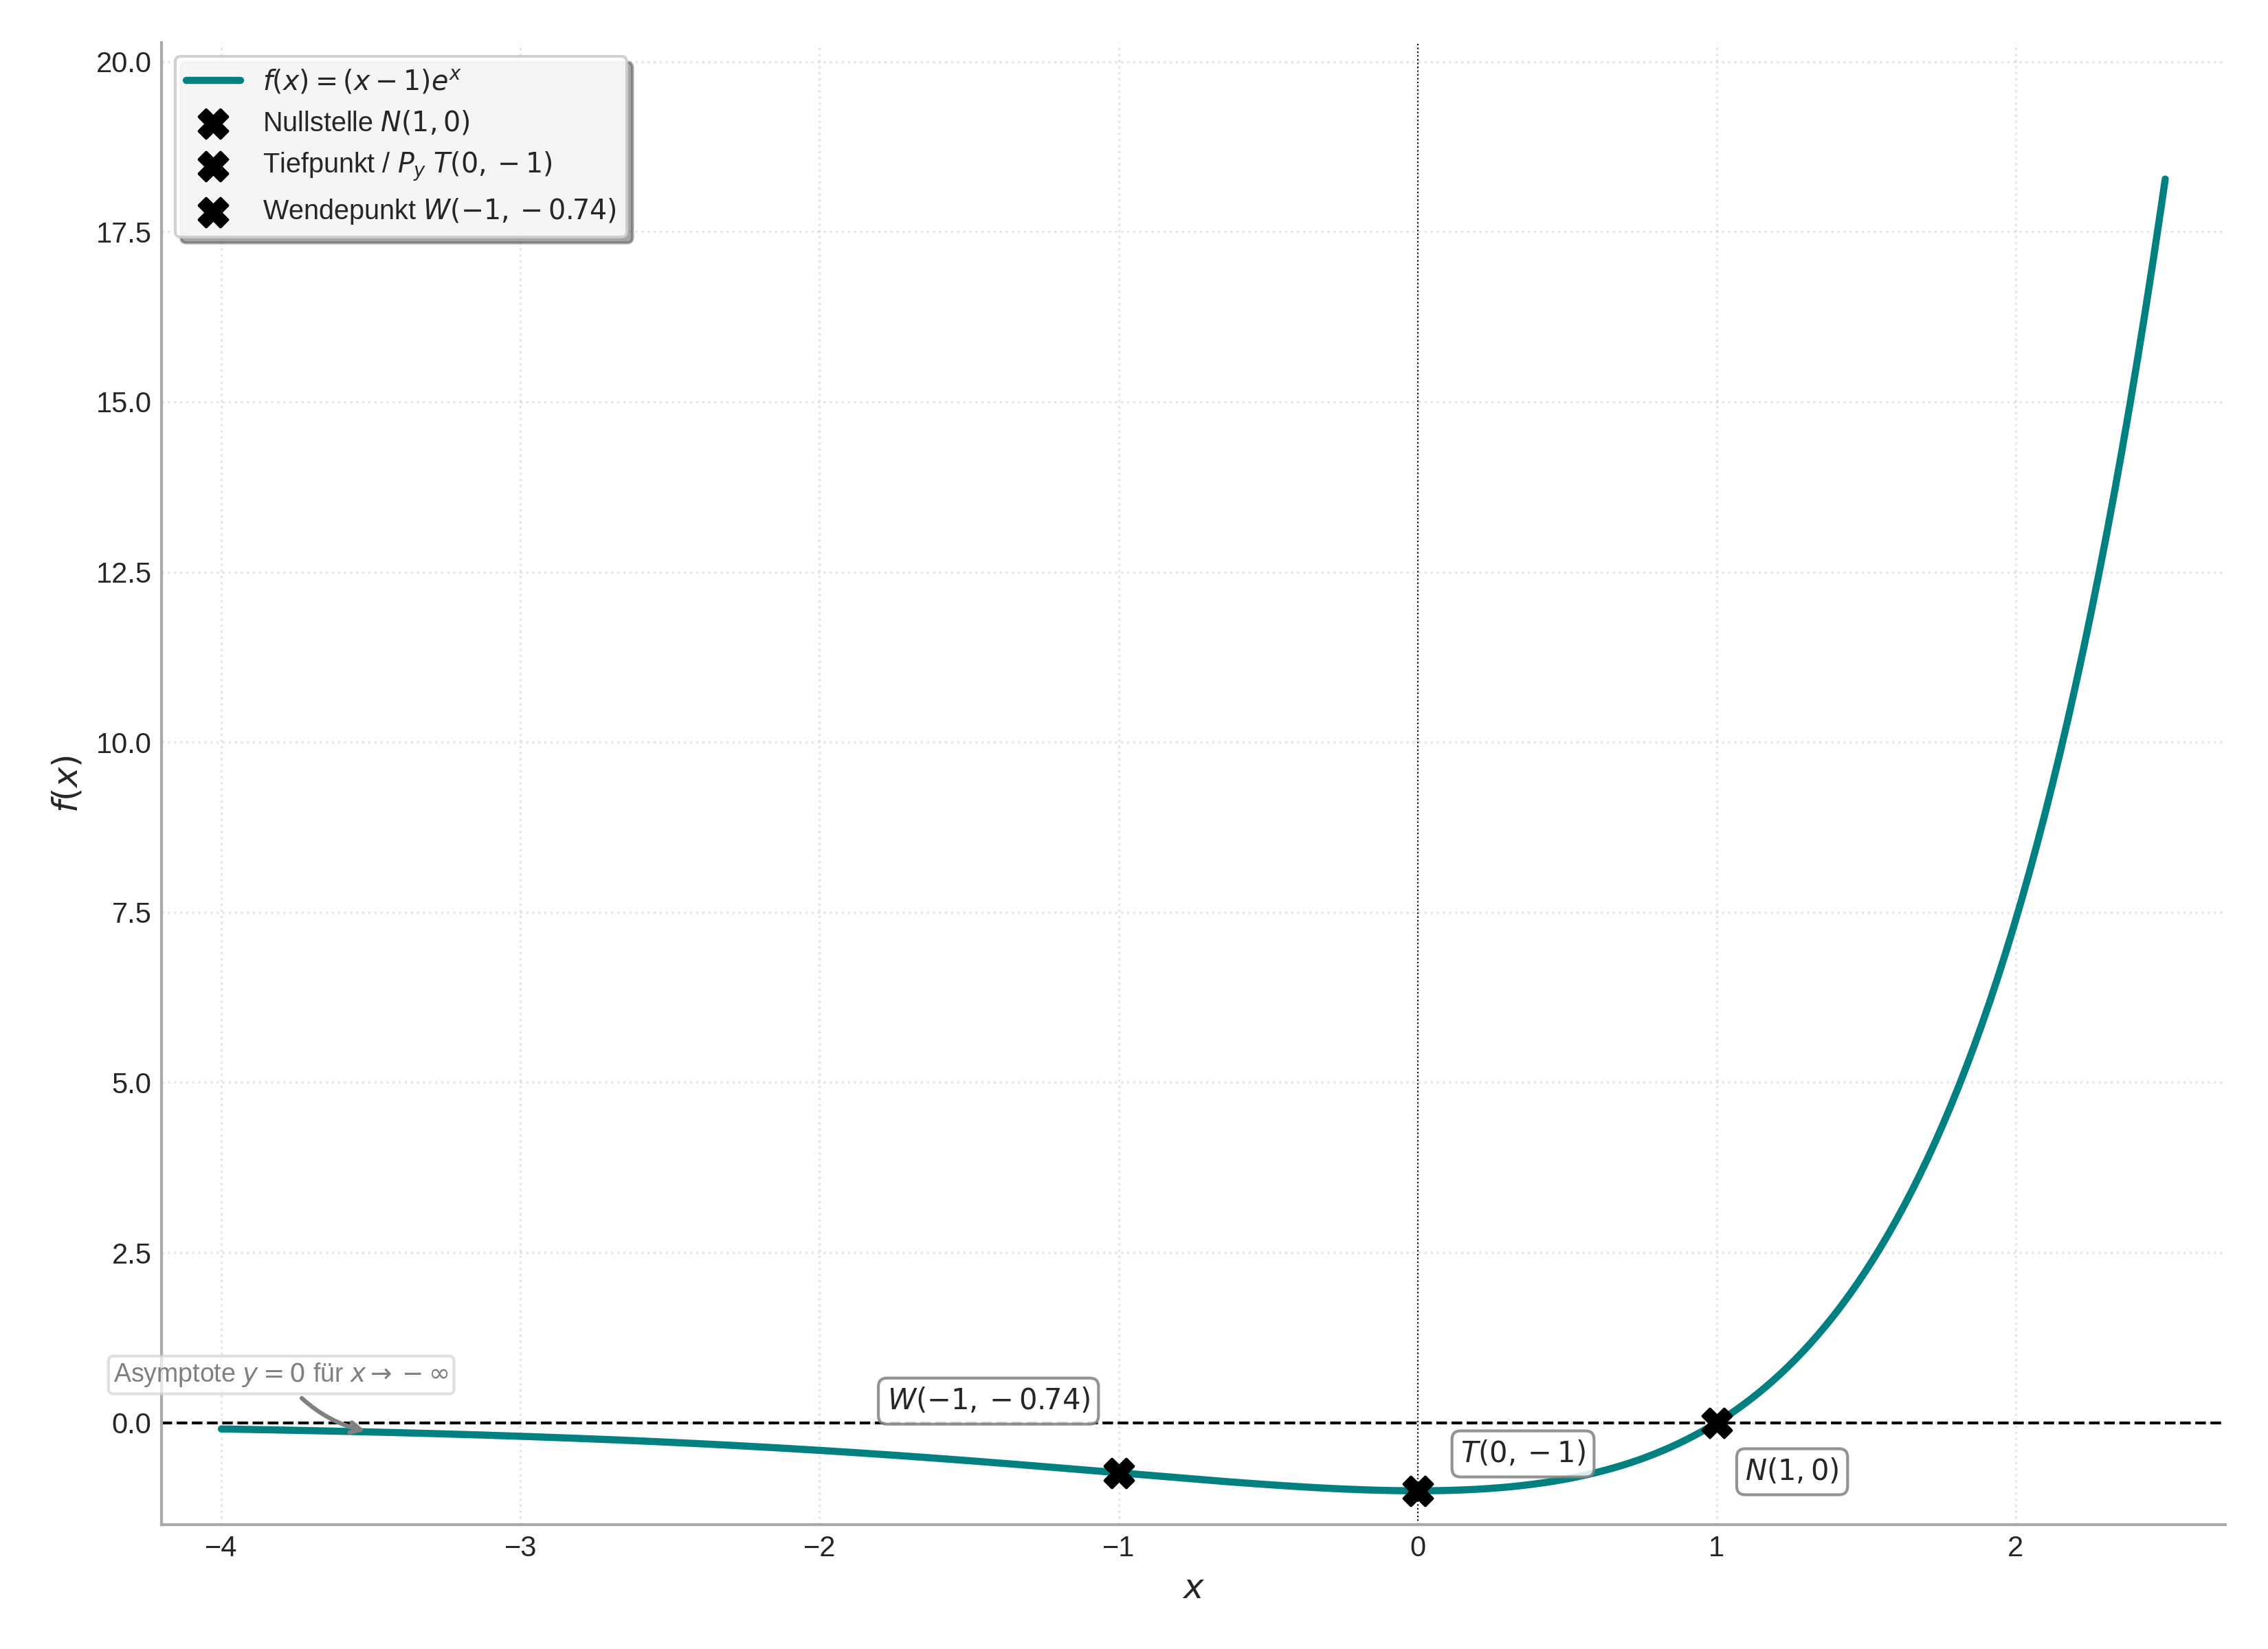
\includegraphics[width=0.9\textwidth]{grafiken/Kurvendiskussion_eFunktion_Polynom.png}
            \captionof{figure}{Graph von $f(x)=(x-1)e^x$}
            \label{fig:kurvendisk_ex_polynom}
        \end{center}
\end{enumerate}
\end{beispielumgebung}


% ... (Nach Beispiel 7.7 und der zugehörigen Abbildung \ref{fig:kurvendisk_ex_polynom}) ...

\begin{infoboxumgebung}{Die Regel von L'Hôpital – Grenzwerte bei '$\frac{0}{0}$' oder '$\frac{\infty}{\infty}$'}
Manchmal stoßen wir bei der Berechnung von Grenzwerten auf unbestimmte Ausdrücke wie '$\frac{0}{0}$' oder '$\frac{\pm\infty}{\pm\infty}$'. Eine direkte Einsetzung des Grenzwertes ist dann nicht möglich. Für solche Fälle gibt es eine elegante Methode, die nach dem französischen Mathematiker Guillaume de L'Hôpital (1661-1704) benannt ist.

\textbf{Die Regel von L'Hôpital:}
Seien $f(x)$ und $g(x)$ zwei differenzierbare Funktionen. Wenn der Grenzwert des Quotienten $\frac{f(x)}{g(x)}$ für $x \to a$ (wobei $a$ eine Zahl, $\infty$ oder $-\infty$ sein kann) einen der folgenden unbestimmten Ausdrücke ergibt:
\begin{itemize}
    \item $\lim_{x \to a} f(x) = 0$ und $\lim_{x \to a} g(x) = 0$ (Fall '$\frac{0}{0}$')
    \item $\lim_{x \to a} f(x) = \pm\infty$ und $\lim_{x \to a} g(x) = \pm\infty$ (Fall '$\frac{\pm\infty}{\pm\infty}$')
\end{itemize}
Dann gilt, vorausgesetzt der Grenzwert auf der rechten Seite existiert (oder ist $\pm\infty$):
\[ \lim_{x \to a} \frac{f(x)}{g(x)} = \lim_{x \to a} \frac{f'(x)}{g'(x)} \]
\textbf{Wichtig:} Man leitet Zähler und Nenner \textbf{getrennt} voneinander ab, nicht mit der Quotientenregel! Die Regel kann bei Bedarf auch mehrfach hintereinander angewendet werden, solange die Voraussetzungen erfüllt sind.

\textbf{Was ist mit dem Fall '$0 \cdot \infty$'?}
Auch diesen unbestimmten Ausdruck kann man oft auf die Form '$\frac{0}{0}$' oder '$\frac{\infty}{\infty}$' bringen, um L'Hôpital anwenden zu können. Zum Beispiel kann man $f(x) \cdot g(x)$ umschreiben zu $\frac{f(x)}{1/g(x)}$ oder $\frac{g(x)}{1/f(x)}$.

\textbf{Beispiele (mit $e^x$ und Polynomen):}
\begin{enumerate}
    \item \textbf{Fall '$\frac{0}{0}$':} $\lim_{x \to 0} \frac{e^x - 1 - x}{x^2}$
        \begin{itemize}
            \item Für $x \to 0$: Zähler $e^0 - 1 - 0 = 1-1-0=0$. Nenner $0^2=0$. (Fall '$\frac{0}{0}$')
            \item Ableitungen: $f(x) = e^x-1-x \implies f'(x) = e^x-1$. $g(x) = x^2 \implies g'(x) = 2x$.
            \item $\lim_{x \to 0} \frac{e^x-1}{2x}$. Für $x \to 0$: Zähler $e^0-1=0$. Nenner $2 \cdot 0=0$. (Wieder '$\frac{0}{0}$')
            \item Erneute Anwendung von L'Hôpital:
            Ableitungen: $(e^x-1)' = e^x$. $(2x)' = 2$.
            \item $\lim_{x \to 0} \frac{e^x}{2} = \frac{e^0}{2} = \frac{1}{2}$.
        \end{itemize}
    \item \textbf{Fall '$\frac{\infty}{\infty}$' und die 'Stärke' von $e^x$:} $\lim_{x \to \infty} \frac{x^2}{e^x}$
        \begin{itemize}
            \item Für $x \to \infty$: Zähler $x^2 \to \infty$. Nenner $e^x \to \infty$. (Fall '$\frac{\infty}{\infty}$')
            \item Ableitungen: $(x^2)' = 2x$. $(e^x)' = e^x$.
            \item $\lim_{x \to \infty} \frac{2x}{e^x}$. Für $x \to \infty$: Zähler $2x \to \infty$. Nenner $e^x \to \infty$. (Wieder '$\frac{\infty}{\infty}$')
            \item Erneute Anwendung von L'Hôpital:
            Ableitungen: $(2x)' = 2$. $(e^x)' = e^x$.
            \item $\lim_{x \to \infty} \frac{2}{e^x}$. Da $e^x \to \infty$, geht der Bruch gegen $0$. Also: $\lim_{x \to \infty} \frac{x^2}{e^x} = 0$.
        \end{itemize}
        \textit{Erklärung zur Dominanz von $e^x$:} Dieses Beispiel zeigt, warum $e^x$ (für $x \to \infty$) 'stärker wächst' als jedes Polynom $x^n$. Bei jeder Anwendung der Regel von L'Hôpital wird der Grad des Polynoms im Zähler um 1 reduziert, bis schließlich eine Konstante übrig bleibt. Die $e^x$-Funktion im Nenner bleibt jedoch bei jeder Ableitung (bis auf eventuelle konstante Faktoren bei $e^{kx}$) im Wesentlichen erhalten und strebt weiterhin gegen $\infty$. Daher wird der Grenzwert des Bruchs letztendlich Null.

    \item \textbf{Fall '$0 \cdot \infty$':} $\lim_{x \to -\infty} x e^x$ (aus Beispiel 7.7)
        \begin{itemize}
            \item Für $x \to -\infty$: $x \to -\infty$ und $e^x \to 0$. (Fall '$-\infty \cdot 0$')
            \item Umformen zu '$\frac{-\infty}{\infty}$': $x e^x = \frac{x}{e^{-x}}$. Für $x \to -\infty$: Zähler $x \to -\infty$. Nenner $e^{-x} \to e^{\infty} \to \infty$.
            \item Ableitungen: $(x)' = 1$. $(e^{-x})' = -e^{-x}$ (Kettenregel).
            \item $\lim_{x \to -\infty} \frac{1}{-e^{-x}}$. Für $x \to -\infty$: Nenner $-e^{-x} \to -e^{\infty} \to -\infty$.
            \item Der Bruch $\frac{1}{-\infty}$ geht gegen $0$. Also: $\lim_{x \to -\infty} x e^x = 0$.
        \end{itemize}
\end{enumerate}
\textbf{Achtung:} Die Regel von L'Hôpital darf nur angewendet werden, wenn tatsächlich einer der unbestimmten Ausdrücke '$\frac{0}{0}$' oder '$\frac{\pm\infty}{\pm\infty}$' vorliegt! Eine falsche Anwendung führt zu falschen Ergebnissen.
\end{infoboxumgebung}


\begin{aufgabenumgebung}{Kurvendiskussionen mit Exponentialfunktionen}
Führe eine vollständige Kurvendiskussion für die folgenden Funktionen durch.
\begin{enumerate}
    \item $f(x) = x e^{-x}$
    \item $g(x) = (x^2-2)e^x$
    \item \textbf{Für Experten:} $h(x) = e^{x^2-2x}$. (Hier wird die Kettenregel komplexer, aber die Struktur der Kurvendiskussion bleibt gleich.)
\end{enumerate}
\end{aufgabenumgebung}

\begin{tippumgebung}{Anwendungsaufgaben mit Exponentialfunktionen}
Exponentialfunktionen sind ideal, um Prozesse zu beschreiben, bei denen die Änderungsrate vom Bestand abhängt.
\begin{itemize}
    \item \textbf{Wachstum:} $N(t) = N_0 \cdot e^{kt}$ mit $k>0$ (z.B. Bakterienkultur, Zinseszins bei stetiger Verzinsung). $N_0$ ist der Anfangsbestand.
    \item \textbf{Zerfall:} $N(t) = N_0 \cdot e^{-kt}$ mit $k>0$ (z.B. radioaktiver Zerfall, Abklingvorgänge). $N_0$ ist der Anfangsbestand. Die Konstante $k$ wird oft als Zerfallskonstante bezeichnet.
    \item \textbf{Logistisches Wachstum (Ausblick):} Für begrenztes Wachstum gibt es komplexere Modelle wie $N(t) = \frac{G}{1+e^{-kG(t-t_0)}}$, die eine Sättigungsgrenze $G$ haben.
\end{itemize}
Bei solchen Aufgaben geht es oft darum, die Parameter ($N_0, k$) aus gegebenen Bedingungen zu bestimmen oder Vorhersagen zu treffen.
\end{tippumgebung}

\begin{aufgabenumgebung}{Anwendung: Radioaktiver Zerfall}
Eine radioaktive Substanz zerfällt so, dass die noch vorhandene Menge $M(t)$ (in Gramm) nach $t$ Jahren durch die Funktion $M(t) = 100 \cdot e^{-0.05t}$ beschrieben wird.
\begin{enumerate}
    \item Wie groß ist die Anfangsmenge der Substanz?
    \item Wie viel Gramm sind nach 10 Jahren noch vorhanden?
    \item Mit welcher Rate zerfällt die Substanz zum Zeitpunkt $t=0$ und zum Zeitpunkt $t=10$ Jahre (in Gramm pro Jahr)? (Tipp: Ableitung $M'(t)$).
    \item \textbf{Halbwertszeit:} Nach welcher Zeit $T_H$ ist nur noch die Hälfte der ursprünglichen Menge vorhanden? (Setze $M(T_H) = \frac{1}{2}M(0)$ und löse nach $T_H$. Hierfür benötigst du den natürlichen Logarithmus $\ln$, die Umkehrfunktion von $e^x$.)
\end{enumerate}
\end{aufgabenumgebung}

% Vorheriger Inhalt des Kapitels bis zur Aufgabe 'Anwendung: Radioaktiver Zerfall'
% ... (siehe vorherige Canvas-Version) ...

\subsubsection{Weitere anspruchsvolle Aufgaben mit Exponentialfunktionen}
\label{subsubsec:exp_anwendungen_vertiefung}

Die folgenden Aufgaben kombinieren die Ableitung von Exponentialfunktionen mit den Konzepten der Kurvendiskussion und Anwendungen. Sie erfordern oft mehrere Ableitungsregeln und ein gutes Verständnis der Zusammenhänge.

\begin{aufgabenumgebung}{Optimierung im biologischen Kontext – Wachstum und Hemmung}
Eine Bakterienpopulation wächst zunächst, wird aber durch einen hemmenden Faktor (z.B. begrenzte Nährstoffe) beeinflusst. Die Anzahl der Bakterien $N$ (in Tausend) nach $t$ Stunden kann modelliert werden durch die Funktion:
\[ N(t) = 5t \cdot e^{-0.1t} \quad (\text{für } t \ge 0) \]
\begin{enumerate}
    \item \textbf{Anfangsbestand:} Wie viele Bakterien sind zum Zeitpunkt $t=0$ vorhanden? Interpretiere das Ergebnis im Kontext.
    \item \textbf{Wachstumsrate:} Bestimme die Funktion $N'(t)$, welche die Wachstumsrate der Bakterienpopulation zum Zeitpunkt $t$ angibt. (Produkt- und Kettenregel sind hier gefragt!)
    \item \textbf{Maximale Population:}
        \begin{itemize}
            \item Zu welchem Zeitpunkt $t_{max}$ erreicht die Bakterienpopulation ihr Maximum? (Tipp: Notwendige Bedingung für Extremstellen $N'(t)=0$. Da $e^{-0.1t}$ nie Null wird, musst du nur den anderen Faktor betrachten.)
            \item Überprüfe mit der zweiten Ableitung $N''(t)$ oder dem Vorzeichenwechselkriterium von $N'(t)$, ob es sich tatsächlich um ein Maximum handelt.
            \item Wie groß ist die maximale Bakterienpopulation $N(t_{max})$?
        \end{itemize}
    \item \textbf{Verhalten für $t \to \infty$:} Was passiert mit der Bakterienpopulation für sehr große Zeiten? (Untersuche $\lim_{t \to \infty} N(t)$). Ist das biologisch sinnvoll?
    \item \textbf{Stärkste Zunahme/Abnahme der Wachstumsrate (für Experten):}
        Die Änderungsrate der Wachstumsrate wird durch $N''(t)$ beschrieben. Wann ist die Zunahme der Wachstumsrate maximal (d.h. wann wächst die Population am schnellsten schneller)? Wann ist die Abnahme der Wachstumsrate maximal (d.h. wann verlangsamt sich das Wachstum am stärksten)? (Tipp: Untersuche $N''(t)$ auf Extremstellen, d.h. bilde $N'''(t)$).
    \item \textbf{Skizze:} Skizziere den Graphen von $N(t)$ für $t \ge 0$ und markiere den maximalen Bestand.
\end{enumerate}
\end{aufgabenumgebung}

\begin{aufgabenumgebung}{Tangenten an Exponentialfunktionen}
Gegeben ist die Funktion $f(x) = (x-2)e^x$.
\begin{enumerate}
    \item Bestimme die Gleichung der Tangente an den Graphen von $f$ im Punkt $P(2|f(2))$.
    \item In welchem Punkt schneidet diese Tangente die y-Achse?
    \item Gibt es eine Stelle $x_0$, an der die Tangente an den Graphen von $f$ parallel zur x-Achse verläuft? Wenn ja, bestimme $x_0$ und die Art des Extrempunktes an dieser Stelle.
    \item (Für Experten): Gibt es eine Tangente an den Graphen von $f$, die durch den Ursprung $(0|0)$ verläuft, aber nicht im Ursprung berührt?
        \begin{tippumgebung}{Tangente durch externen Punkt}
        Sei $B(x_B | f(x_B))$ der unbekannte Berührpunkt der Tangente am Graphen. Die Steigung der Tangente ist $m_T = f'(x_B)$. Die Tangente geht auch durch den Ursprung $O(0|0)$. Die Steigung der Geraden durch $O$ und $B$ ist auch $\frac{f(x_B)-0}{x_B-0}$. Setze diese beiden Ausdrücke für die Steigung gleich: $f'(x_B) = \frac{f(x_B)}{x_B}$. Löse diese Gleichung nach $x_B$.
        \end{tippumgebung}
\end{enumerate}
\end{aufgabenumgebung}

\begin{aufgabenumgebung}{Kurvendiskussion einer komplexeren e-Funktion}
Führe eine vollständige Kurvendiskussion für die Funktion $f(x) = (x^2 - 3)e^{-x}$ durch. Untersuche dabei insbesondere:
\begin{itemize}
    \item Definitionsbereich, Symmetrie
    \item Verhalten im Unendlichen (Grenzwerte, Asymptoten)
    \item Nullstellen
    \item Extrempunkte (Lage und Art)
    \item Wendepunkte (Lage)
    \item Skizziere den Graphen von $f(x)$.
\end{itemize}
\begin{tippumgebung}{Ableitungen}
Du wirst hier die Produkt- und Kettenregel mehrfach anwenden müssen. Achte auf sorgfältiges Rechnen und Vereinfachen. Das Ausklammern von $e^{-x}$ (oder $e^{\text{irgendwas}}$) ist oft hilfreich!
\end{tippumgebung}
\end{aufgabenumgebung}

% Vorheriger Inhalt des Kapitels bis zur aufgabenumgebung 'Der Mittelwert einer Funktion'
% ... (siehe vorherige Canvas-Version) ...

\subsection{Weitere Integrationstechniken – Mehr als nur Polynome aufleiten}
\label{subsec:integrationstechniken}

Bisher haben wir uns hauptsächlich mit der Integration (dem Aufleiten) von Polynomfunktionen und einfachen Potenzfunktionen beschäftigt, bei denen die Umkehrung der Potenz-, Faktor- und Summenregel der Ableitung ausreichte. Doch was machen wir, wenn wir komplexere Funktionen integrieren wollen, zum Beispiel Produkte von Funktionen oder verkettete Funktionen, wie sie uns oft bei Exponentialfunktionen begegnen?

Für solche Fälle benötigen wir erweiterte Integrationstechniken. Zwei der wichtigsten sind die \textbf{partielle Integration} (die Umkehrung der Produktregel der Ableitung) und die \textbf{Integration durch Substitution} (die Umkehrung der Kettenregel der Ableitung).

\subsubsection{Partielle Integration – Die 'Produktregel rückwärts'}
\label{subsubsec:partielle_integration}

Die Produktregel der Ableitung lautet: $(u(x) \cdot v(x))' = u'(x)v(x) + u(x)v'(x)$.
Wenn wir diese Gleichung auf beiden Seiten integrieren und umstellen, erhalten wir die Formel für die partielle Integration. Sie ist besonders nützlich, wenn der Integrand ein Produkt aus zwei Funktionen ist, von denen eine beim Ableiten 'einfacher' wird und die andere leicht zu integrieren ist.

\begin{merksatzumgebung}{Partielle Integration}
Wenn $u(x)$ und $v(x)$ differenzierbare Funktionen sind, dann gilt:
\[ \int u'(x) \cdot v(x) \,dx = u(x) \cdot v(x) - \int u(x) \cdot v'(x) \,dx \]
Oder, wenn man $f(x) = u(x)$ und $g'(x) = v'(x)$ setzt, also $g(x) = v(x)$:
\[ \int f(x) \cdot g'(x) \,dx = f(x) \cdot g(x) - \int f'(x) \cdot g(x) \,dx \]
Die Kunst besteht darin, den Integranden geschickt in einen Faktor $u'(x)$ (der leicht zu $u(x)$ integriert werden kann) und einen Faktor $v(x)$ (dessen Ableitung $v'(x)$ das neue Integral vereinfacht) zu zerlegen.
\end{merksatzumgebung}

\begin{tippumgebung}{Wahl von $u'(x)$ und $v(x)$ bei partieller Integration}
Eine Faustregel (die nicht immer gilt, aber oft hilft):
\begin{itemize}
    \item Wähle $v(x)$ so, dass seine Ableitung $v'(x)$ 'einfacher' wird als $v(x)$ selbst (z.B. Polynome, deren Grad sich beim Ableiten verringert).
    \item Wähle $u'(x)$ so, dass du es leicht zu $u(x)$ integrieren (aufleiten) kannst.
\end{itemize}
Manchmal muss man die partielle Integration auch mehrfach hintereinander anwenden.
\end{tippumgebung}

\begin{beispielumgebung}{Partielle Integration mit $e^x$}
Wir wollen das Integral $\int x \cdot e^x \,dx$ berechnen.
Dies ist ein Produkt aus $x$ und $e^x$.

\textbf{Schritt 1: Wähle $u'(x)$ und $v(x)$.}
Eine gute Wahl ist oft, den Polynomterm als $v(x)$ zu wählen, da er beim Ableiten einfacher wird.
Sei $v(x) = x \implies v'(x) = 1$.
Dann muss $u'(x) = e^x \implies u(x) = \int e^x \,dx = e^x$. (Wir können die Integrationskonstante hier weglassen, da sie am Ende sowieso als Gesamtkonstante $C$ erscheint).

\textbf{Schritt 2: Setze in die Formel $\int u'(x)v(x) \,dx = u(x)v(x) - \int u(x)v'(x) \,dx$ ein.}
(Beachte: Unsere Wahl war $v(x)$ und $u'(x)$, die Formel ist aber oft mit $u(x)$ und $v'(x)$ notiert. Wir passen uns hier der ersten Formel im Merksatz an, indem wir $u'(x)$ und $v(x)$ identifizieren. Alternativ könnten wir $f(x)=x$ und $g'(x)=e^x$ setzen.)

Nehmen wir die zweite Formel im Merksatz: $\int f(x) \cdot g'(x) \,dx = f(x) \cdot g(x) - \int f'(x) \cdot g(x) \,dx$.
Wähle:
$f(x) = x \implies f'(x) = 1$.
$g'(x) = e^x \implies g(x) = e^x$.

Dann ist $\int x \cdot e^x \,dx = x \cdot e^x - \int 1 \cdot e^x \,dx$.

\textbf{Schritt 3: Löse das verbleibende Integral.}
$\int 1 \cdot e^x \,dx = \int e^x \,dx = e^x$.

\textbf{Schritt 4: Setze alles zusammen und füge die Integrationskonstante $C$ hinzu.}
$\int x \cdot e^x \,dx = x e^x - e^x + C = e^x(x-1) + C$.

\textit{Probe durch Ableiten des Ergebnisses $F(x) = e^x(x-1) + C$:}
$F'(x) = (e^x(x-1))' + (C)'$. Für den ersten Term nutzen wir die Produktregel:
$u(x)=e^x \implies u'(x)=e^x$
$v(x)=x-1 \implies v'(x)=1$
$(e^x(x-1))' = e^x(x-1) + e^x(1) = xe^x - e^x + e^x = xe^x$.
Also $F'(x) = xe^x + 0 = xe^x$. Das ist unser ursprünglicher Integrand!
\end{beispielumgebung}

\begin{fehlerboxumgebung}{Partielle Integration – Häufige Fehlerquellen}
Die partielle Integration ist ein sehr nützliches Werkzeug, aber achte auf diese typischen Stolpersteine:
\begin{itemize}
    \item \textbf{Ungünstige Wahl von $f(x)$ und $g'(x)$ (bzw. $v(x)$ und $u'(x)$):}
    Wenn das neue Integral $\int f'(x)g(x) \,dx$ komplizierter oder zumindest nicht einfacher als das Ausgangsintegral wird, war die Wahl der zu differenzierenden und zu integrierenden Teile oft nicht optimal. Orientiere dich an der Faustregel aus der Tipp-Box (Polynomanteile werden durch Ableiten meist einfacher). Manchmal muss man auch einfach eine Wahl ausprobieren.

    \item \textbf{Fehler beim Ableiten von $f(x)$ oder Integrieren von $g'(x)$:}
    Eine falsche Ableitung $f'(x)$ oder eine falsch gebildete Stammfunktion $g(x)$ führt unweigerlich zu einem falschen Endergebnis. Überprüfe diese Teilschritte sorgfältig!

    \item \textbf{Vorzeichenfehler in der Hauptformel:}
    Die Formel lautet $\int f(x) g'(x) \,dx = f(x)g(x) - \int f'(x)g(x) \,dx$. Das \textbf{Minuszeichen} vor dem zweiten Integral ist entscheidend und wird leicht vergessen oder durch ein Plus ersetzt.

    \item \textbf{Das Integralzeichen beim zweiten Term vergessen:}
    Es ist wichtig, dass der zweite Term auf der rechten Seite immer noch ein Integral ist: $f(x)g(x) - \mathbf{\int} f'(x)g(x) \,dx$. Ein häufiger Fehler ist, das Integralzeichen hier wegzulassen und nur $f(x)g(x) - f'(x)g(x)$ zu rechnen.

    \item \textbf{Verwechslung der Terme in der Formel:}
    Achte genau darauf, welche Funktion abgeleitet ($f'(x)$) und welche als Stammfunktion ($g(x)$) in den jeweiligen Teilen der Formel eingesetzt wird. Eine sorgfältige Notation hilft hier.

    \item \textbf{Integrationskonstante $C$ am Ende vergessen:}
    Auch wenn man die Integrationskonstante bei der Bildung der Stammfunktion $g(x)$ im Zwischenschritt meist weglässt, darf sie beim Endergebnis des unbestimmten Integrals nicht fehlen: $\dots + C$.

    \item \textbf{Fehler bei mehrfacher partieller Integration:}
    Muss die partielle Integration mehrmals angewendet werden (z.B. bei $\int x^2 e^x \,dx$), ist es besonders wichtig, Klammern korrekt zu setzen und Vorzeichenfehler zu vermeiden, da sich Fehler leicht fortpflanzen.
\end{itemize}
Gehe bei der partiellen Integration immer sehr systematisch und konzentriert vor!
\end{fehlerboxumgebung}


\begin{aufgabenumgebung}{Partielle Integration üben – Mehr Vielfalt}
Berechne die folgenden unbestimmten Integrale mit partieller Integration:
\begin{enumerate}
    \item $\int (2x+1)e^x \,dx$
    \item $\int x^2 e^x \,dx$ (Tipp: Hier musst du die partielle Integration zweimal anwenden!)
    \item $\int \ln(x) \,dx$
        \begin{tippumgebung}{Umgang mit $\ln(x)$}
        Wähle für die partielle Integration $f(x)=\ln(x)$ und $g'(x)=1$. Du benötigst die Ableitung von $\ln(x)$, die $(\ln x)' = \frac{1}{x}$ ist. (Der natürliche Logarithmus $\ln(x)$ ist die Umkehrfunktion zur $e$-Funktion, mehr dazu im nächsten Kapitel!)
        \end{tippumgebung}
    \item $\int x \cos(x) \,dx$
        \begin{tippumgebung}{Sinus und Kosinus – Ableiten und Aufleiten}
        Auch wenn wir trigonometrische Funktionen erst später ausführlich behandeln, hier die benötigten Informationen:
        \begin{itemize}
            \item Ableitungen: $(\sin x)' = \cos x$ und $(\cos x)' = -\sin x$.
            \item Stammfunktionen: $\int \sin x \,dx = -\cos x + C$ und $\int \cos x \,dx = \sin x + C$.
        \end{itemize}
        Wähle $f(x)=x$ und $g'(x)=\cos x$.
        \end{tippumgebung}
    \item $\int (x^2+1)\ln(x) \,dx$
        \begin{tippumgebung}{Polynom mal Logarithmus}
        Wähle wieder $f(x)=\ln(x)$ und $g'(x)=x^2+1$. (Nutze $(\ln x)' = \frac{1}{x}$).
        \end{tippumgebung}
    \item \textbf{Herausforderung (das 'Trick-Integral'):} $\int e^x \sin(x) \,dx$
        \begin{tippumgebung}{Zweimal partiell integrieren und umstellen}
        \begin{enumerate}
            \item Wende die partielle Integration einmal an (z.B. mit $f(x)=\sin x$ und $g'(x)=e^x$). Das neue Integral wird $e^x \cos(x)$ (oder ähnlich) enthalten.
            \item Wende auf dieses neue Integral \textit{noch einmal} die partielle Integration an (wähle deine Faktoren konsistent, z.B. wieder den trigonometrischen Teil zum Ableiten).
            \item Du solltest nun eine Gleichung erhalten, in der das ursprüngliche Integral $\int e^x \sin(x) \,dx$ auf beiden Seiten vorkommt. Stelle diese Gleichung nach dem gesuchten Integral um! Nutze die Ableitungen/Stammfunktionen für Sinus und Kosinus aus dem vorherigen Tipp.
        \end{enumerate}
        Dieser Typ von Integral ist ein Klassiker!
        \end{tippumgebung}
\end{enumerate}
\end{aufgabenumgebung}

\subsubsection{Integration durch Substitution – Die 'Kettenregel rückwärts'}
\label{subsubsec:integration_substitution}

Die Integration durch Substitution ist eine mächtige Technik, die besonders dann hilfreich ist, wenn der Integrand eine verkettete Funktion enthält und gleichzeitig die Ableitung der inneren Funktion als Faktor auftaucht (oder leicht dorthin gebracht werden kann). Sie ist die Umkehrung der Kettenregel der Ableitung: $(g(h(x)))' = g'(h(x)) \cdot h'(x)$.

\begin{merksatzumgebung}{Integration durch Substitution}
Wenn wir ein Integral der Form $\int f(g(x)) \cdot g'(x) \,dx$ haben, können wir substituieren (ersetzen):
\begin{enumerate}
    \item Setze $u = g(x)$ (die innere Funktion).
    \item Bilde die Ableitung von $u$ nach $x$: $\frac{du}{dx} = g'(x)$.
    \item Stelle dies nach $dx$ um (formal): $du = g'(x)dx$.
    \item Ersetze $g(x)$ durch $u$ und $g'(x)dx$ durch $du$ im Integral.
    \item Integriere den neuen Ausdruck nach $u$: $\int f(u) \,du = F(u) + C$.
    \item \textbf{Rücksubstituiere}: Ersetze $u$ wieder durch $g(x)$, um das Ergebnis in Abhängigkeit von $x$ zu erhalten: $F(g(x)) + C$.
\end{enumerate}
Kurz: $\int f(g(x)) \cdot g'(x) \,dx = \int f(u) \,du = F(u) + C = F(g(x)) + C$.
\end{merksatzumgebung}

\begin{tippumgebung}{Wann Substitution anwenden?}
Suche im Integranden nach einer 'inneren Funktion' $g(x)$, deren Ableitung $g'(x)$ (oder ein Vielfaches davon) ebenfalls als Faktor im Integranden vorkommt.
\end{tippumgebung}

\begin{beispielumgebung}{Integration durch Substitution mit $e^x$}
\begin{enumerate}
    \item \textbf{Integral $\int e^{3x+2} \,dx$}
        Hier ist die innere Funktion $g(x) = 3x+2$.
        \begin{itemize}
            \item Substitution: $u = 3x+2$.
            \item Ableiten von $u$: $\frac{du}{dx} = 3$.
            \item Nach $dx$ umstellen: $du = 3dx \implies dx = \frac{1}{3}du$.
            \item Einsetzen ins Integral: $\int e^u \cdot \frac{1}{3}du = \frac{1}{3} \int e^u \,du$.
            \item Integrieren nach $u$: $\frac{1}{3} e^u + C$.
            \item Rücksubstituieren ($u=3x+2$): $\frac{1}{3}e^{3x+2} + C$.
        \end{itemize}
        Das bestätigt unsere frühere Regel $\int e^{kx}dx = \frac{1}{k}e^{kx}+C$ für $k=3$.

    \item \textbf{Integral $\int 2x \cdot e^{x^2-1} \,dx$}
        Hier ist die innere Funktion im Exponenten $g(x) = x^2-1$. Ihre Ableitung ist $g'(x)=2x$. Dieser Faktor $2x$ steht praktischerweise schon vor dem $e$-Term!
        \begin{itemize}
            \item Substitution: $u = x^2-1$.
            \item Ableiten von $u$: $\frac{du}{dx} = 2x$.
            \item Umstellen: $du = 2x \,dx$.
            \item Einsetzen: Der Term $e^{x^2-1}$ wird zu $e^u$, und der Term $2x \,dx$ wird zu $du$.
            Das Integral wird zu $\int e^u \,du$.
            \item Integrieren nach $u$: $e^u + C$.
            \item Rücksubstituieren ($u=x^2-1$): $e^{x^2-1} + C$.
        \end{itemize}
        \textit{Probe durch Ableiten:} $(e^{x^2-1}+C)'$. Äußere Fkt: $e^u$, innere Fkt: $u=x^2-1$.
        Ableitung: $e^{x^2-1} \cdot (2x) = 2x e^{x^2-1}$. Stimmt!
\end{enumerate}
\end{beispielumgebung}

\begin{fehlerboxumgebung}{Integrieren von $e^{kx}$ und $b^x$}
Auch beim Aufleiten (Integrieren) von Exponentialfunktionen gibt es typische Stolpersteine:
\begin{itemize}
    \item \textbf{Faktor $\frac{1}{k}$ beim Integrieren von $e^{kx}$ vergessen:} Die Stammfunktion von $f(x)=e^{kx}$ ist $F(x) = \frac{1}{k}e^{kx} + C$. Der Faktor $\frac{1}{k}$ (Kehrwert der inneren Ableitung) ist wichtig!
    \textit{Beispiel Falsch:} $\int e^{2x} \,dx = e^{2x} + C$. \textit{Richtig:} $\int e^{2x} \,dx = \frac{1}{2}e^{2x} + C$.
    \item \textbf{Faktor $\frac{1}{\ln(b)}$ beim Integrieren von $b^x$ vergessen:} Die Stammfunktion von $f(x)=b^x$ ist $F(x) = \frac{1}{\ln(b)}b^x + C$.
    \textit{Beispiel Falsch:} $\int 2^x \,dx = 2^x + C$. \textit{Richtig:} $\int 2^x \,dx = \frac{1}{\ln(2)}2^x + C$.
    \item \textbf{Vorzeichenfehler bei negativem $k$ oder $0 < b < 1$:} Wenn $k$ negativ ist (z.B. $e^{-3x}$), wird $\frac{1}{k}$ ebenfalls negativ. Wenn $0 < b < 1$, ist $\ln(b)$ negativ. Achte hier sorgfältig auf die Vorzeichen.
\end{itemize}
Überprüfe deine Stammfunktionen immer durch Ableiten!
\end{fehlerboxumgebung}

\begin{aufgabenumgebung}{Integration durch Substitution – Vielfältige Übungen}
Berechne die folgenden unbestimmten Integrale mit der Substitutionsmethode:
\begin{enumerate}
    \item $\int (2x+1)^4 \,dx$ (Tipp: $u=2x+1$)
    \item $\int x \cdot e^{x^2} \,dx$ (Tipp: $u=x^2$. Was ist $du$? Du musst eventuell einen Faktor anpassen.)
    \item $\int \frac{1}{(3x-5)^2} \,dx$ (Tipp: Schreibe als $(3x-5)^{-2}$ und substituiere $u=3x-5$)
    \item $\int \cos(2x) \,dx$ (Stammfunktion von $\cos(u)$ ist $\sin(u)$. Substituiere $u=2x$.)
    \item $\int 3x^2 \cdot (x^3+7)^5 \,dx$ 
        \begin{tippumgebung}{Innere Funktion und ihre Ableitung}
        Wähle $u=x^3+7$. Was ist die Ableitung $u' = \frac{du}{dx}$? Kommt dieser Term (oder ein Vielfaches) im Integranden vor?
        \end{tippumgebung}
    \item $\int \sqrt{4x-3} \,dx$ 
        \begin{tippumgebung}{Wurzel als Potenz}
        Schreibe $\sqrt{4x-3}$ als $(4x-3)^{\frac{1}{2}}$ und substituiere $u=4x-3$.
        \end{tippumgebung}
    \item $\int \frac{5x}{(x^2-1)^3} \,dx$
        \begin{tippumgebung}{Konstanter Faktor}
        Wähle $u=x^2-1$. Dann ist $du = 2x \,dx$. Der Faktor $x$ ist also Teil von $du$. Den konstanten Faktor 5 kannst du vor das Integral ziehen und den Faktor 2 (von $2x$) durch einen Faktor $\frac{1}{2}$ ausgleichen.
        \end{tippumgebung}
    \item $\int (x+2) \cdot e^{x^2+4x-1} \,dx$
        \begin{tippumgebung}{Exponent als innere Funktion}
        Substituiere den gesamten Exponenten $u=x^2+4x-1$. Prüfe, ob die Ableitung $u'$ (oder ein Vielfaches davon) als Faktor im Integranden vorhanden ist.
        \end{tippumgebung}
    \item \textbf{Herausforderung:} $\int \frac{x^3}{\sqrt{1+x^4}} \,dx$
        \begin{tippumgebung}{Substitution unter der Wurzel}
        Substituiere $u=1+x^4$. Beachte, dass $du = 4x^3 \,dx$ ist. Du musst also den Faktor $\frac{1}{4}$ ergänzen. Der Term wird dann zu $\int \frac{1}{4} \cdot u^{-\frac{1}{2}} \,du$.
        \end{tippumgebung}
\end{enumerate}
\end{aufgabenumgebung}

\begin{fehlerboxumgebung}{Häufige Fehler bei der Substitution}
\begin{itemize}
    \item \textbf{$dx$ nicht korrekt ersetzt:} Es reicht nicht, nur $g(x)$ durch $u$ zu ersetzen. Das Differential $dx$ muss auch durch einen Ausdruck mit $du$ ersetzt werden ($dx = \frac{1}{g'(x)}du$).
    \item \textbf{Innere Ableitung $g'(x)$ fehlt oder passt nicht:} Die Methode funktioniert am einfachsten, wenn $g'(x)$ (oder ein Vielfaches davon) bereits als Faktor im Integranden vorhanden ist. Manchmal muss man das Integral geschickt um einen konstanten Faktor erweitern und kürzen.
    \item \textbf{Rücksubstitution vergessen:} Das Endergebnis muss wieder von $x$ abhängen, nicht von $u$!
\end{itemize}
\end{fehlerboxumgebung}

\begin{kurzknappumgebung}{Integrationstechniken für Produkte und Verkettungen}
\begin{itemize}
    \item \textbf{Partielle Integration $\int u'v \,dx = uv - \int uv' \,dx$:}
        Gut für Produkte, bei denen ein Faktor beim Ableiten einfacher wird (z.B. $x^n$) und der andere leicht zu integrieren ist (z.B. $e^x, \sin x, \cos x$).
    \item \textbf{Integration durch Substitution $\int f(g(x))g'(x) \,dx = F(g(x))+C$:}
        Gut für verkettete Funktionen, wenn die Ableitung der inneren Funktion $g'(x)$ als Faktor im Integranden auftaucht.
\end{itemize}
Diese Techniken erweitern unsere Möglichkeiten, Stammfunktionen zu finden, erheblich!
\end{kurzknappumgebung}

\begin{aufgabenumgebung}{Anwendungsaufgabe: Fläche unter $xe^{-x}$}
Die Funktion $f(x) = xe^{-x}$ spielt in einigen Anwendungsbereichen eine Rolle.
\begin{enumerate}
    \item Bestimme die Stammfunktion $F(x)$ von $f(x)$ mithilfe partieller Integration.
    \item Berechne den Inhalt der Fläche, die der Graph von $f(x)$ mit der x-Achse im Intervall $[0, 2]$ einschließt. (Hinweis: Untersuche, ob $f(x)$ im Intervall positiv ist. $e^{-x}$ ist immer positiv).
    \item (Für Experten): Untersuche das Verhalten von $f(x)$ für $x \to \infty$. (Tipp: $\lim_{x \to \infty} xe^{-x} = \lim_{x \to \infty} \frac{x}{e^x} = 0$). Was bedeutet das für die Fläche unter dem Graphen von $x=0$ bis 'unendlich'? Solche Integrale nennt man \textit{uneigentliche Integrale}.
\end{enumerate}
\begin{center}
    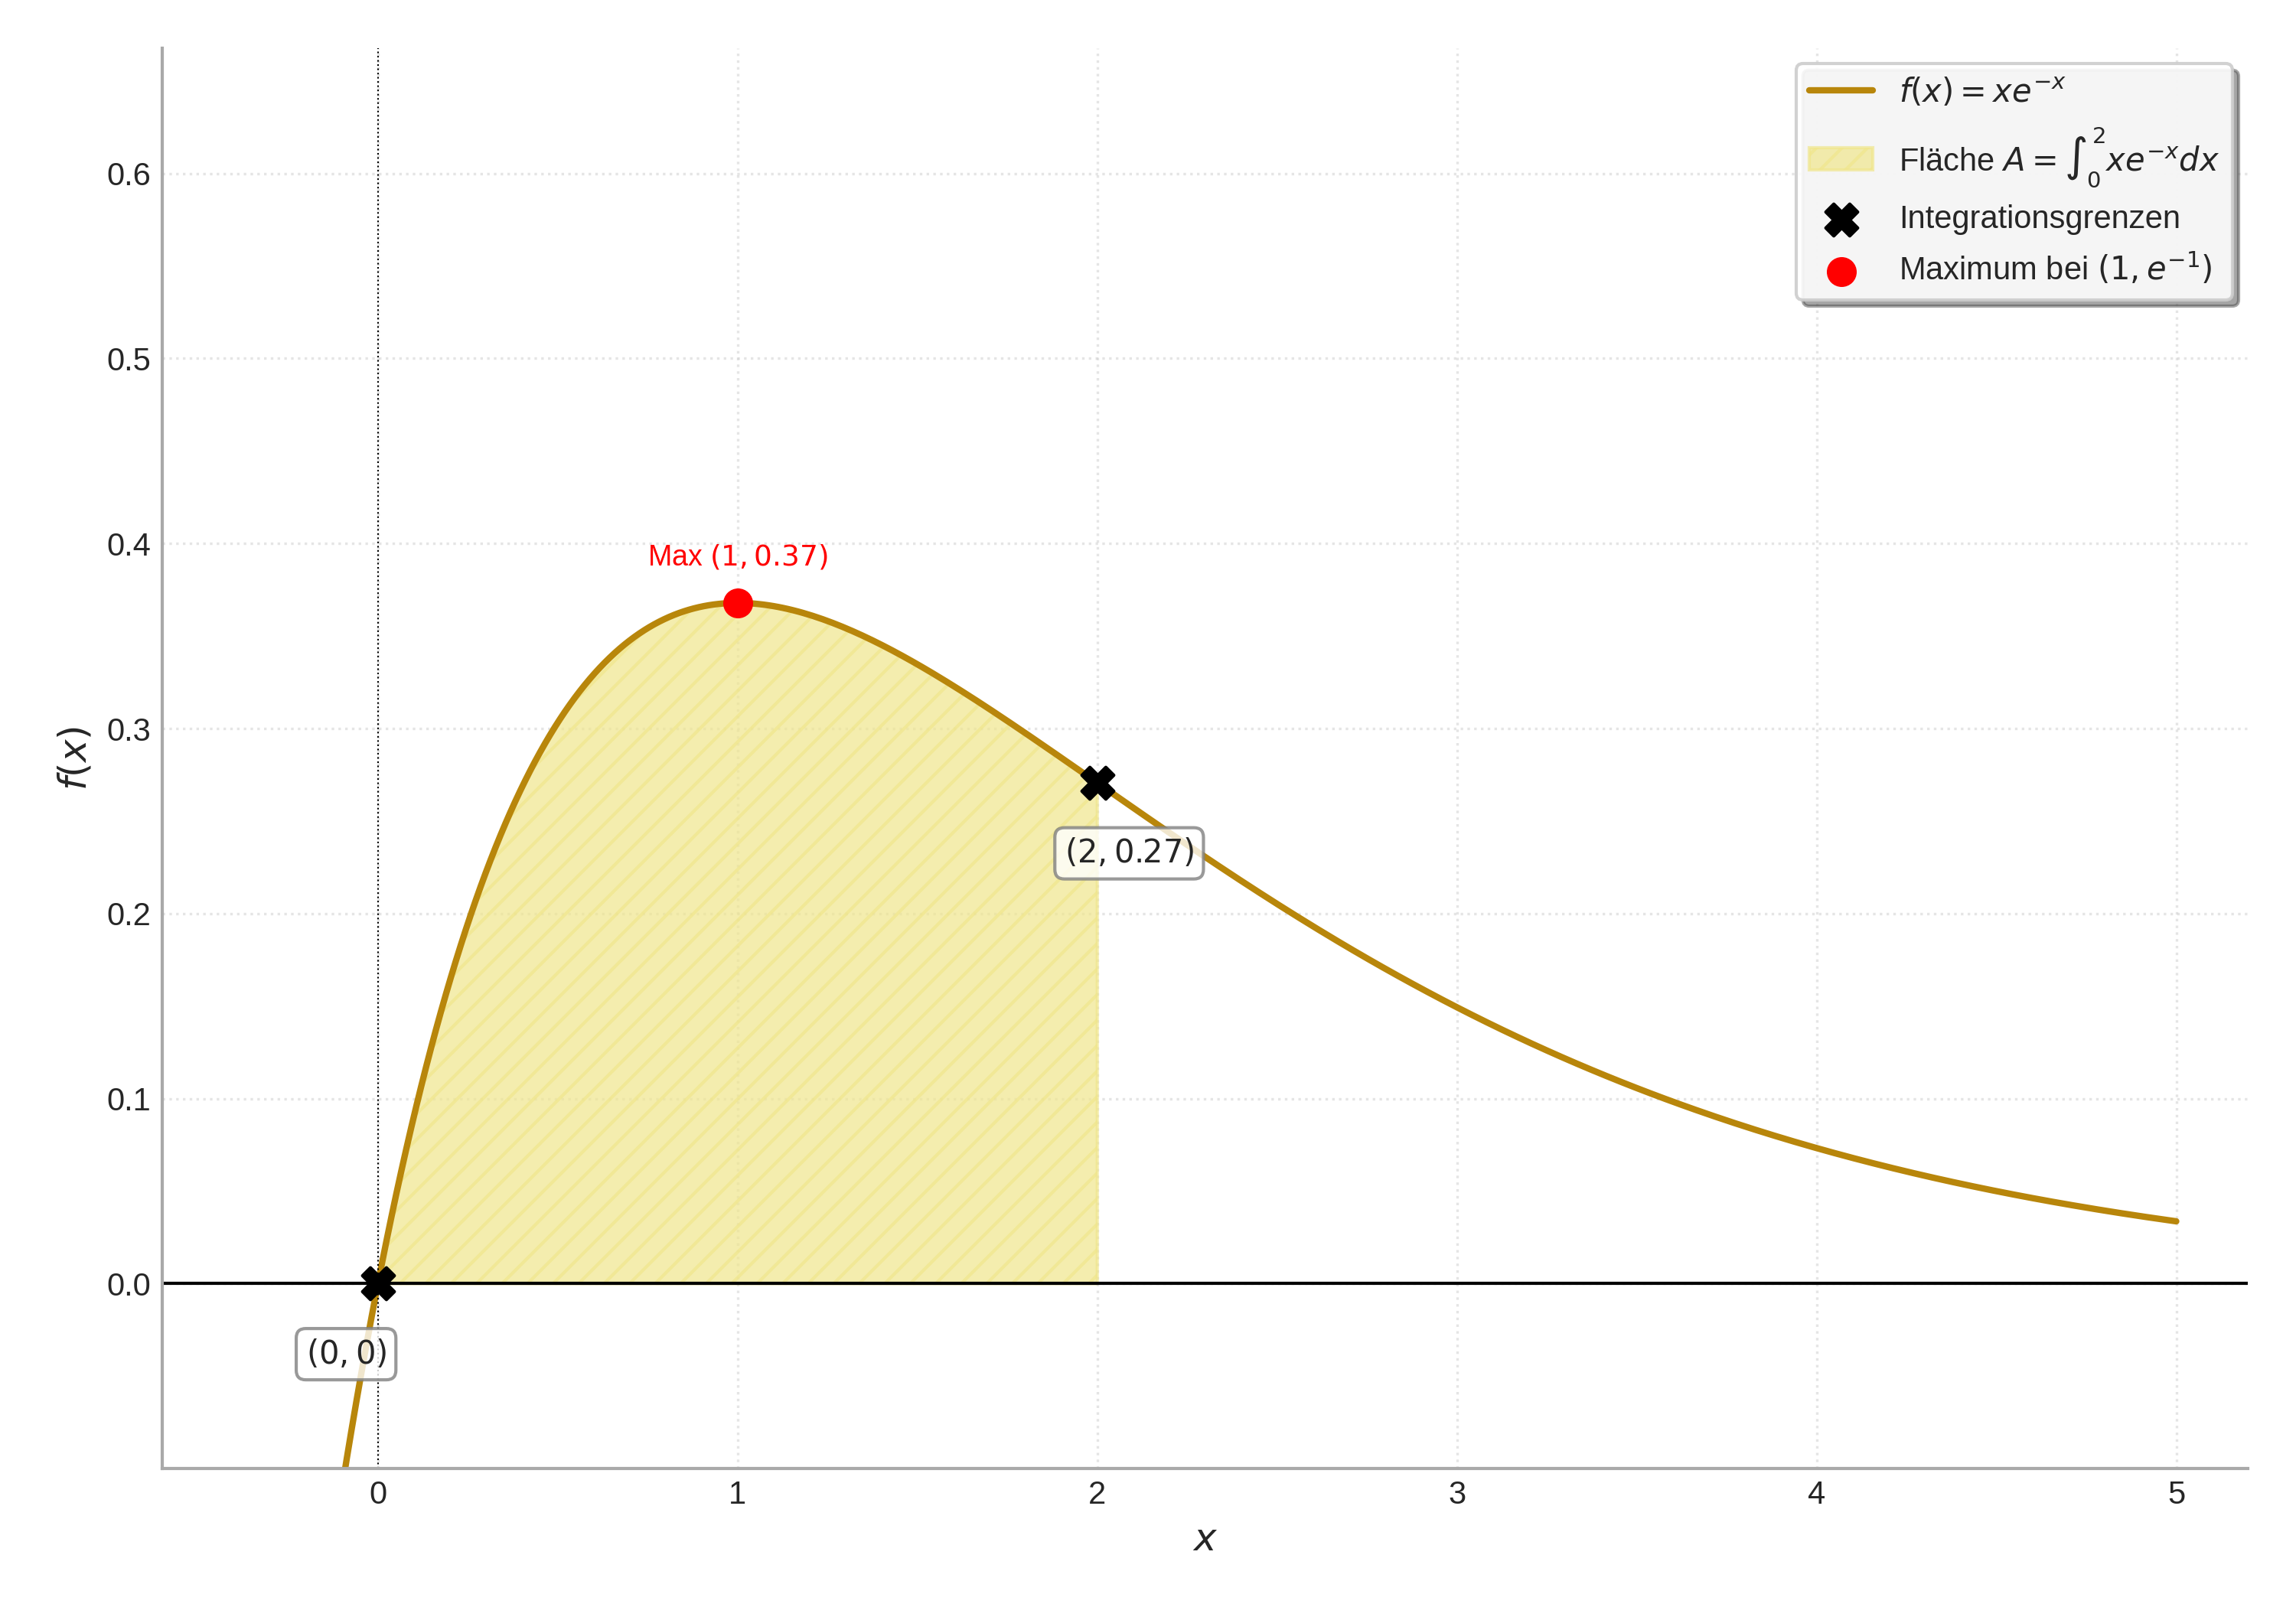
\includegraphics[width=0.8\textwidth]{grafiken/Integral_Flaeche_xehochminusx.png}
    \captionof{figure}{Fläche unter $f(x)=xe^{-x}$}
    \label{fig:flaeche_xehochminusx}
\end{center}
\end{aufgabenumgebung}

% Vorheriger Inhalt des Kapitels bis zur aufgabenumgebung 'Tangentenprobleme an einer kubischen Funktion'
% ... (siehe vorherige Canvas-Version) ...
\subsubsection{Weitere anspruchsvolle Aufgaben mit Exponentialfunktionen}
\label{subsubsec:exp_anwendungen_vertiefung_neu}

Die folgenden Aufgaben kombinieren die Ableitung von Exponentialfunktionen mit den Konzepten der Kurvendiskussion und Anwendungen. Sie erfordern oft mehrere Ableitungsregeln und ein gutes Verständnis der Zusammenhänge.

\begin{aufgabenumgebung}{Optimierung im biologischen Kontext – Wachstum und Hemmung}
Eine Bakterienpopulation wächst zunächst, wird aber durch einen hemmenden Faktor (z.B. begrenzte Nährstoffe) beeinflusst. Die Anzahl der Bakterien $N$ (in Tausend) nach $t$ Stunden kann modelliert werden durch die Funktion:
\[ N(t) = 5t \cdot e^{-0.1t} \quad (\text{für } t \ge 0) \]
\begin{enumerate}
    \item \textbf{Anfangsbestand:} Wie viele Bakterien sind zum Zeitpunkt $t=0$ vorhanden? Interpretiere das Ergebnis im Kontext.
    \item \textbf{Wachstumsrate:} Bestimme die Funktion $N'(t)$, welche die Wachstumsrate der Bakterienpopulation zum Zeitpunkt $t$ angibt. (Produkt- und Kettenregel sind hier gefragt!)
    \item \textbf{Maximale Population:}
        \begin{itemize}
            \item Zu welchem Zeitpunkt $t_{max}$ erreicht die Bakterienpopulation ihr Maximum? (Tipp: Notwendige Bedingung für Extremstellen $N'(t)=0$. Da $e^{-0.1t}$ nie Null wird, musst du nur den anderen Faktor betrachten.)
            \item Überprüfe mit der zweiten Ableitung $N''(t)$ oder dem Vorzeichenwechselkriterium von $N'(t)$, ob es sich tatsächlich um ein Maximum handelt.
            \item Wie groß ist die maximale Bakterienpopulation $N(t_{max})$?
        \end{itemize}
    \item \textbf{Verhalten für $t \to \infty$:} Was passiert mit der Bakterienpopulation für sehr große Zeiten? (Untersuche $\lim_{t \to \infty} N(t)$). Ist das biologisch sinnvoll?
    \item \textbf{Stärkste Zunahme/Abnahme der Wachstumsrate (für Experten):}
        Die Änderungsrate der Wachstumsrate wird durch $N''(t)$ beschrieben. Wann ist die Zunahme der Wachstumsrate maximal (d.h. wann wächst die Population am schnellsten schneller)? Wann ist die Abnahme der Wachstumsrate maximal (d.h. wann verlangsamt sich das Wachstum am stärksten)? (Tipp: Untersuche $N''(t)$ auf Extremstellen, d.h. bilde $N'''(t)$).
    \item \textbf{Skizze:} Skizziere den Graphen von $N(t)$ für $t \ge 0$ und markiere den maximalen Bestand.
\end{enumerate}
\end{aufgabenumgebung}


\subsubsection{Anwendungen der Integralrechnung auf Exponentialfunktionen}
\label{subsubsec:exp_integration_anwendungen}

Nachdem wir gelernt haben, wie man Exponentialfunktionen ableitet und ihre Graphen analysiert, wollen wir nun unser Wissen über die Integralrechnung anwenden. Insbesondere die Berechnung von Flächeninhalten, die von Exponentialfunktionen begrenzt werden, oder die Rekonstruktion von Gesamtbeständen aus exponentiellen Änderungsraten sind wichtige Anwendungen.

Erinnerung an die Stammfunktionen:
\begin{itemize}
    \item $\int e^x \,dx = e^x + C$
    \item $\int e^{kx} \,dx = \frac{1}{k} e^{kx} + C$ (für $k \neq 0$)
    \item Für Produkte wie $x \cdot e^x$ oder $x^2 \cdot e^x$ benötigen wir die partielle Integration.
    \item Für verkettete Funktionen im Exponenten, wie $e^{x^2}$, benötigen wir oft die Substitution (wenn der Faktor $g'(x)$ vorhanden ist).
\end{itemize}

\begin{aufgabenumgebung}{Flächenberechnung mit Exponentialfunktionen}
\begin{enumerate}
    \item \textbf{Fläche unter $e^x$:}
        Berechne den Inhalt der Fläche, die vom Graphen der Funktion $f(x) = e^x$, der x-Achse und den Geraden $x=0$ und $x=2$ eingeschlossen wird. Fertige eine Skizze an und markiere die Fläche.
    \item \textbf{Fläche unter $e^{-x}$:}
        Berechne den Inhalt der Fläche, die vom Graphen der Funktion $g(x) = 2e^{-0.5x}$, der x-Achse und den Geraden $x=0$ und $x=4$ eingeschlossen wird. Skizziere auch hier den Graphen und die Fläche.
    \item \textbf{Fläche zwischen $e^x$ und einer Geraden (für Experten):}
        Die Graphen der Funktionen $f(x) = e^x$ und $h(x) = e\cdot x + 1$ schließen eine Fläche ein.
        \begin{itemize}
            \item Zeige, dass sich die Graphen an der Stelle $x=0$ und $x=1$ schneiden.
            \item Bestimme, welche Funktion im Intervall $[0,1]$ oben bzw. unten liegt.
            \item Berechne den Inhalt der eingeschlossenen Fläche.
                \begin{center}
                    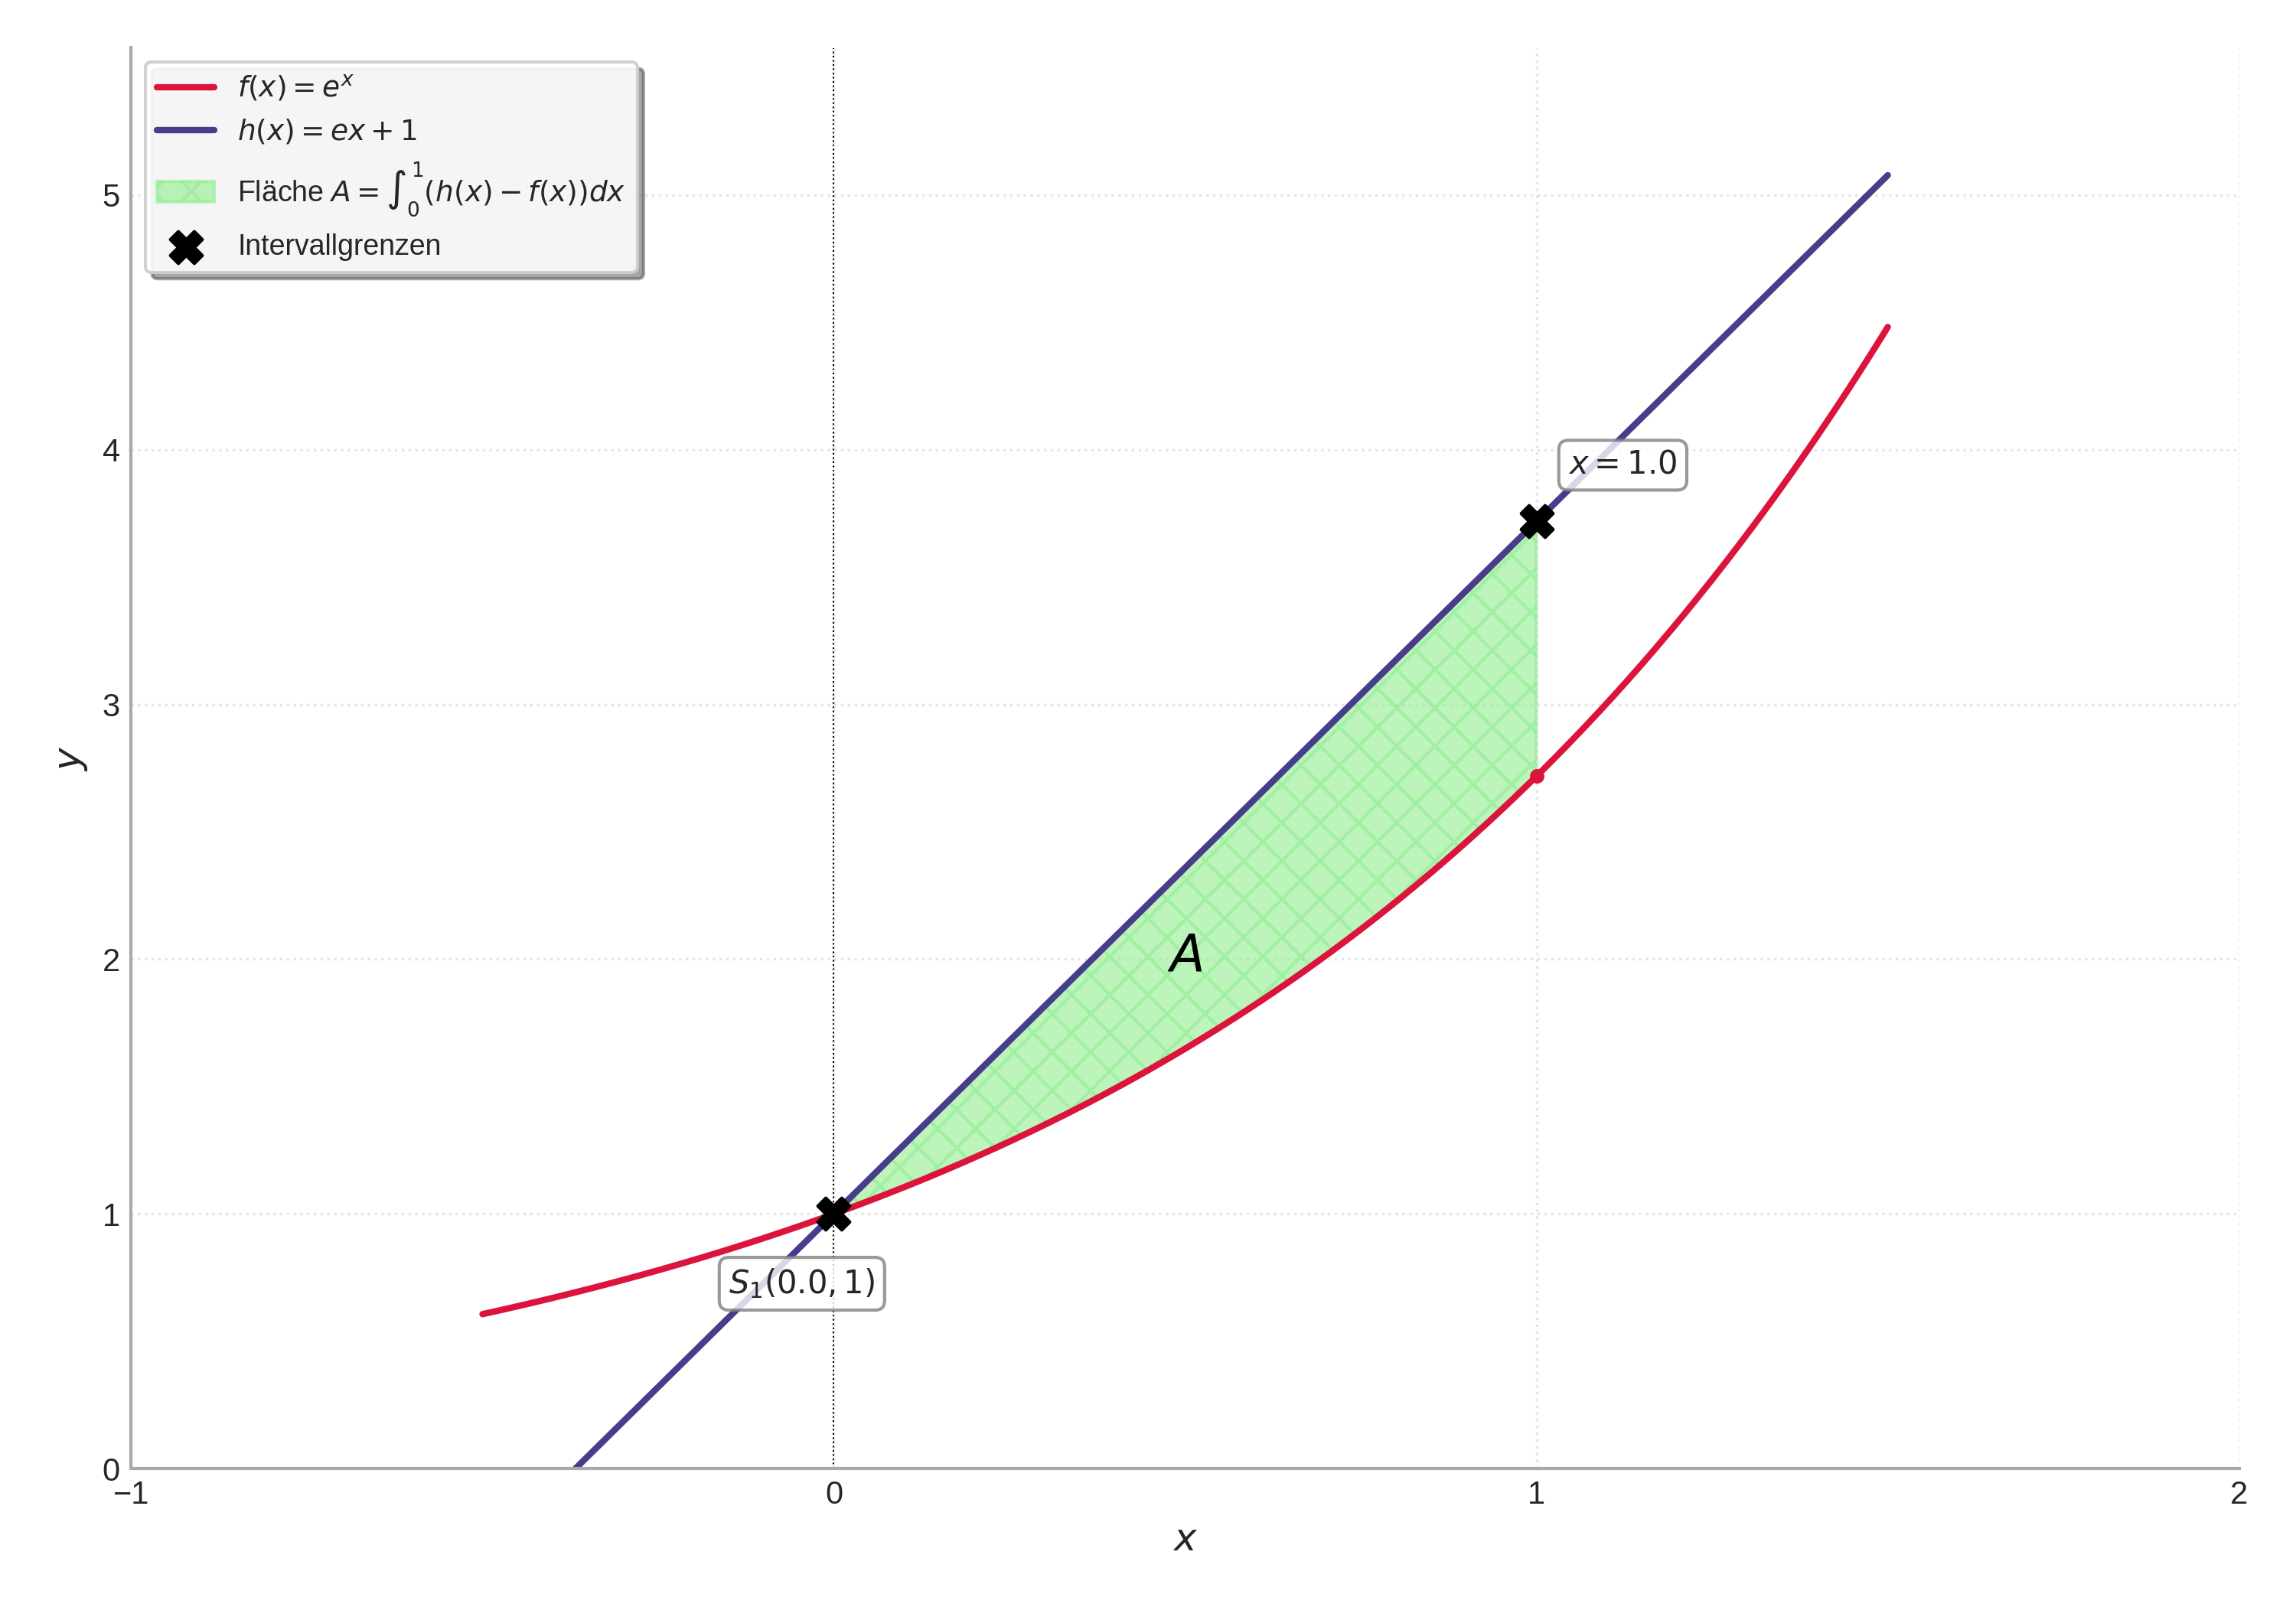
\includegraphics[width=0.8\textwidth]{grafiken/Integral_Flaeche_ex_Gerade.png}
                    \captionof{figure}{Fläche zwischen $f(x)=e^x$ und $h(x)=ex+1$}
                    \label{fig:flaeche_ex_gerade}
                \end{center}
        \end{itemize}
\end{enumerate}
\end{aufgabenumgebung}

\begin{aufgabenumgebung}{Anwendung: Medikamentenabbau im Körper}
Die Konzentration eines Medikaments im Blut eines Patienten (in mg/Liter) kann nach der Einnahme durch die Funktion $K(t) = 10 \cdot t \cdot e^{-0.2t}$ beschrieben werden, wobei $t$ die Zeit in Stunden nach der Einnahme ist ($t \ge 0$).
\begin{enumerate}
    \item Zu welchem Zeitpunkt ist die Konzentration des Medikaments maximal? Wie hoch ist diese maximale Konzentration? (Nutze die Differentialrechnung).
    \item Die 'Gesamtwirkung' eines Medikaments über einen bestimmten Zeitraum kann manchmal durch das Integral der Konzentrationsfunktion über diesen Zeitraum angenähert werden (dies ist eine Vereinfachung, aber das Integral gibt eine Art 'kumulierte Dosis' an).
        Berechne $\int_0^{10} K(t) \,dt$. (Tipp: Partielle Integration ist hier notwendig! Wähle $u'(t)=e^{-0.2t}$ und $v(t)=10t$).
        Was könnte dieser Wert im Kontext bedeuten?
    \item (Für Experten): Was ist $\lim_{t \to \infty} K(t)$? Was bedeutet das für die Konzentration des Medikaments nach sehr langer Zeit?
\end{enumerate}
\end{aufgabenumgebung}

\begin{aufgabenumgebung}{Uneigentliches Integral – Fläche bis ins Unendliche?}
Wir betrachten die Funktion $f(x) = e^{-x}$ für $x \ge 0$.
\begin{enumerate}
    \item Skizziere den Graphen von $f(x)$.
    \item Berechne den Flächeninhalt $A_b = \int_0^b e^{-x} \,dx$ für eine beliebige obere Grenze $b > 0$.
    \item Was passiert mit diesem Flächeninhalt $A_b$, wenn $b$ unendlich groß wird? Berechne also den Grenzwert $\lim_{b \to \infty} A_b$.
    \begin{tippumgebung}{Uneigentliches Integral}
    Ein Integral der Form $\int_a^\infty f(x) \,dx$ nennt man ein \textbf{uneigentliches Integral}. Man berechnet es als Grenzwert:
    \[ \int_a^\infty f(x) \,dx = \lim_{b \to \infty} \int_a^b f(x) \,dx \]
    Wenn dieser Grenzwert existiert (also eine endliche Zahl ist), sagt man, das uneigentliche Integral \textbf{konvergiert}. Ansonsten \textbf{divergiert} es.
    \end{tippumgebung}
    \item Kann eine Fläche, die sich ins Unendliche erstreckt, einen endlichen Inhalt haben? Diskutiere dein Ergebnis aus c).
\end{enumerate}
\end{aufgabenumgebung}



\begin{aufgabenumgebung}{Exponentialfunktionen – Übergreifende und anspruchsvolle Aufgaben}
Die folgenden Aufgaben sollen dein Verständnis für Exponentialfunktionen, ihre Ableitungen, Stammfunktionen und Anwendungen umfassend prüfen. Versuche, die Aufgaben sorgfältig und schrittweise zu lösen.
\begin{enumerate}
    \item \textbf{Kurvendiskussion einer e-Funktion mit Polynomfaktor:}
        Führe eine vollständige Kurvendiskussion für die Funktion $f(x) = (4-x^2)e^{-0.5x}$ durch. Untersuche dabei insbesondere:
        \begin{itemize}
            \item Definitionsbereich und Symmetrie.
            \item Verhalten im Unendlichen und Asymptoten. (Tipp: $\lim_{x\to\infty} x^n e^{-kx} = 0$ für $k>0$).
            \item Nullstellen.
            \item Extrempunkte (Lage und Art).
            \item Wendepunkte (Lage und Krümmungsverhalten).
            \item Skizziere den Graphen von $f(x)$.
        \end{itemize}

    \item \textbf{Optimierung: Maximale Konzentration eines Medikaments}
        Die Konzentration $K(t)$ eines Medikaments im Blut eines Patienten (in mg/l) zum Zeitpunkt $t$ (in Stunden nach Einnahme) wird durch die Funktion $K(t) = 20t \cdot e^{-0.25t}$ für $t \ge 0$ beschrieben.
        \begin{itemize}
            \item Zu welchem Zeitpunkt $t_{max}$ erreicht die Konzentration des Medikaments ihr Maximum?
            \item Wie hoch ist diese maximale Konzentration?
            \item Bestimme die Funktion $K'(t)$, die die Änderungsrate der Konzentration angibt. Wann nimmt die Konzentration am stärksten zu? (Suche nach dem Maximum von $K'(t)$, also einem Wendepunkt von $K(t)$ mit bestimmten Eigenschaften).
        \end{itemize}

    \item \textbf{Flächenberechnung und uneigentliches Integral:}
        Gegeben ist die Funktion $f(x) = (x+1)e^{-x}$.
        \begin{itemize}
            \item Bestimme die Stammfunktion $F(x)$ von $f(x)$ mithilfe partieller Integration.
            \item Berechne den Inhalt der Fläche, die der Graph von $f(x)$ mit der x-Achse und der y-Achse im ersten Quadranten einschließt. (Finde dazu die Nullstelle von $f(x)$ für $x \ge 0$).
            \item (Für Experten): Untersuche, ob die Fläche, die der Graph von $f(x)$ mit der x-Achse für $x \ge 0$ einschließt, einen endlichen Inhalt hat. Berechne dazu das uneigentliche Integral $\int_0^\infty (x+1)e^{-x} \,dx = \lim_{b \to \infty} \int_0^b (x+1)e^{-x} \,dx$.
        \end{itemize}
            \begin{center}
                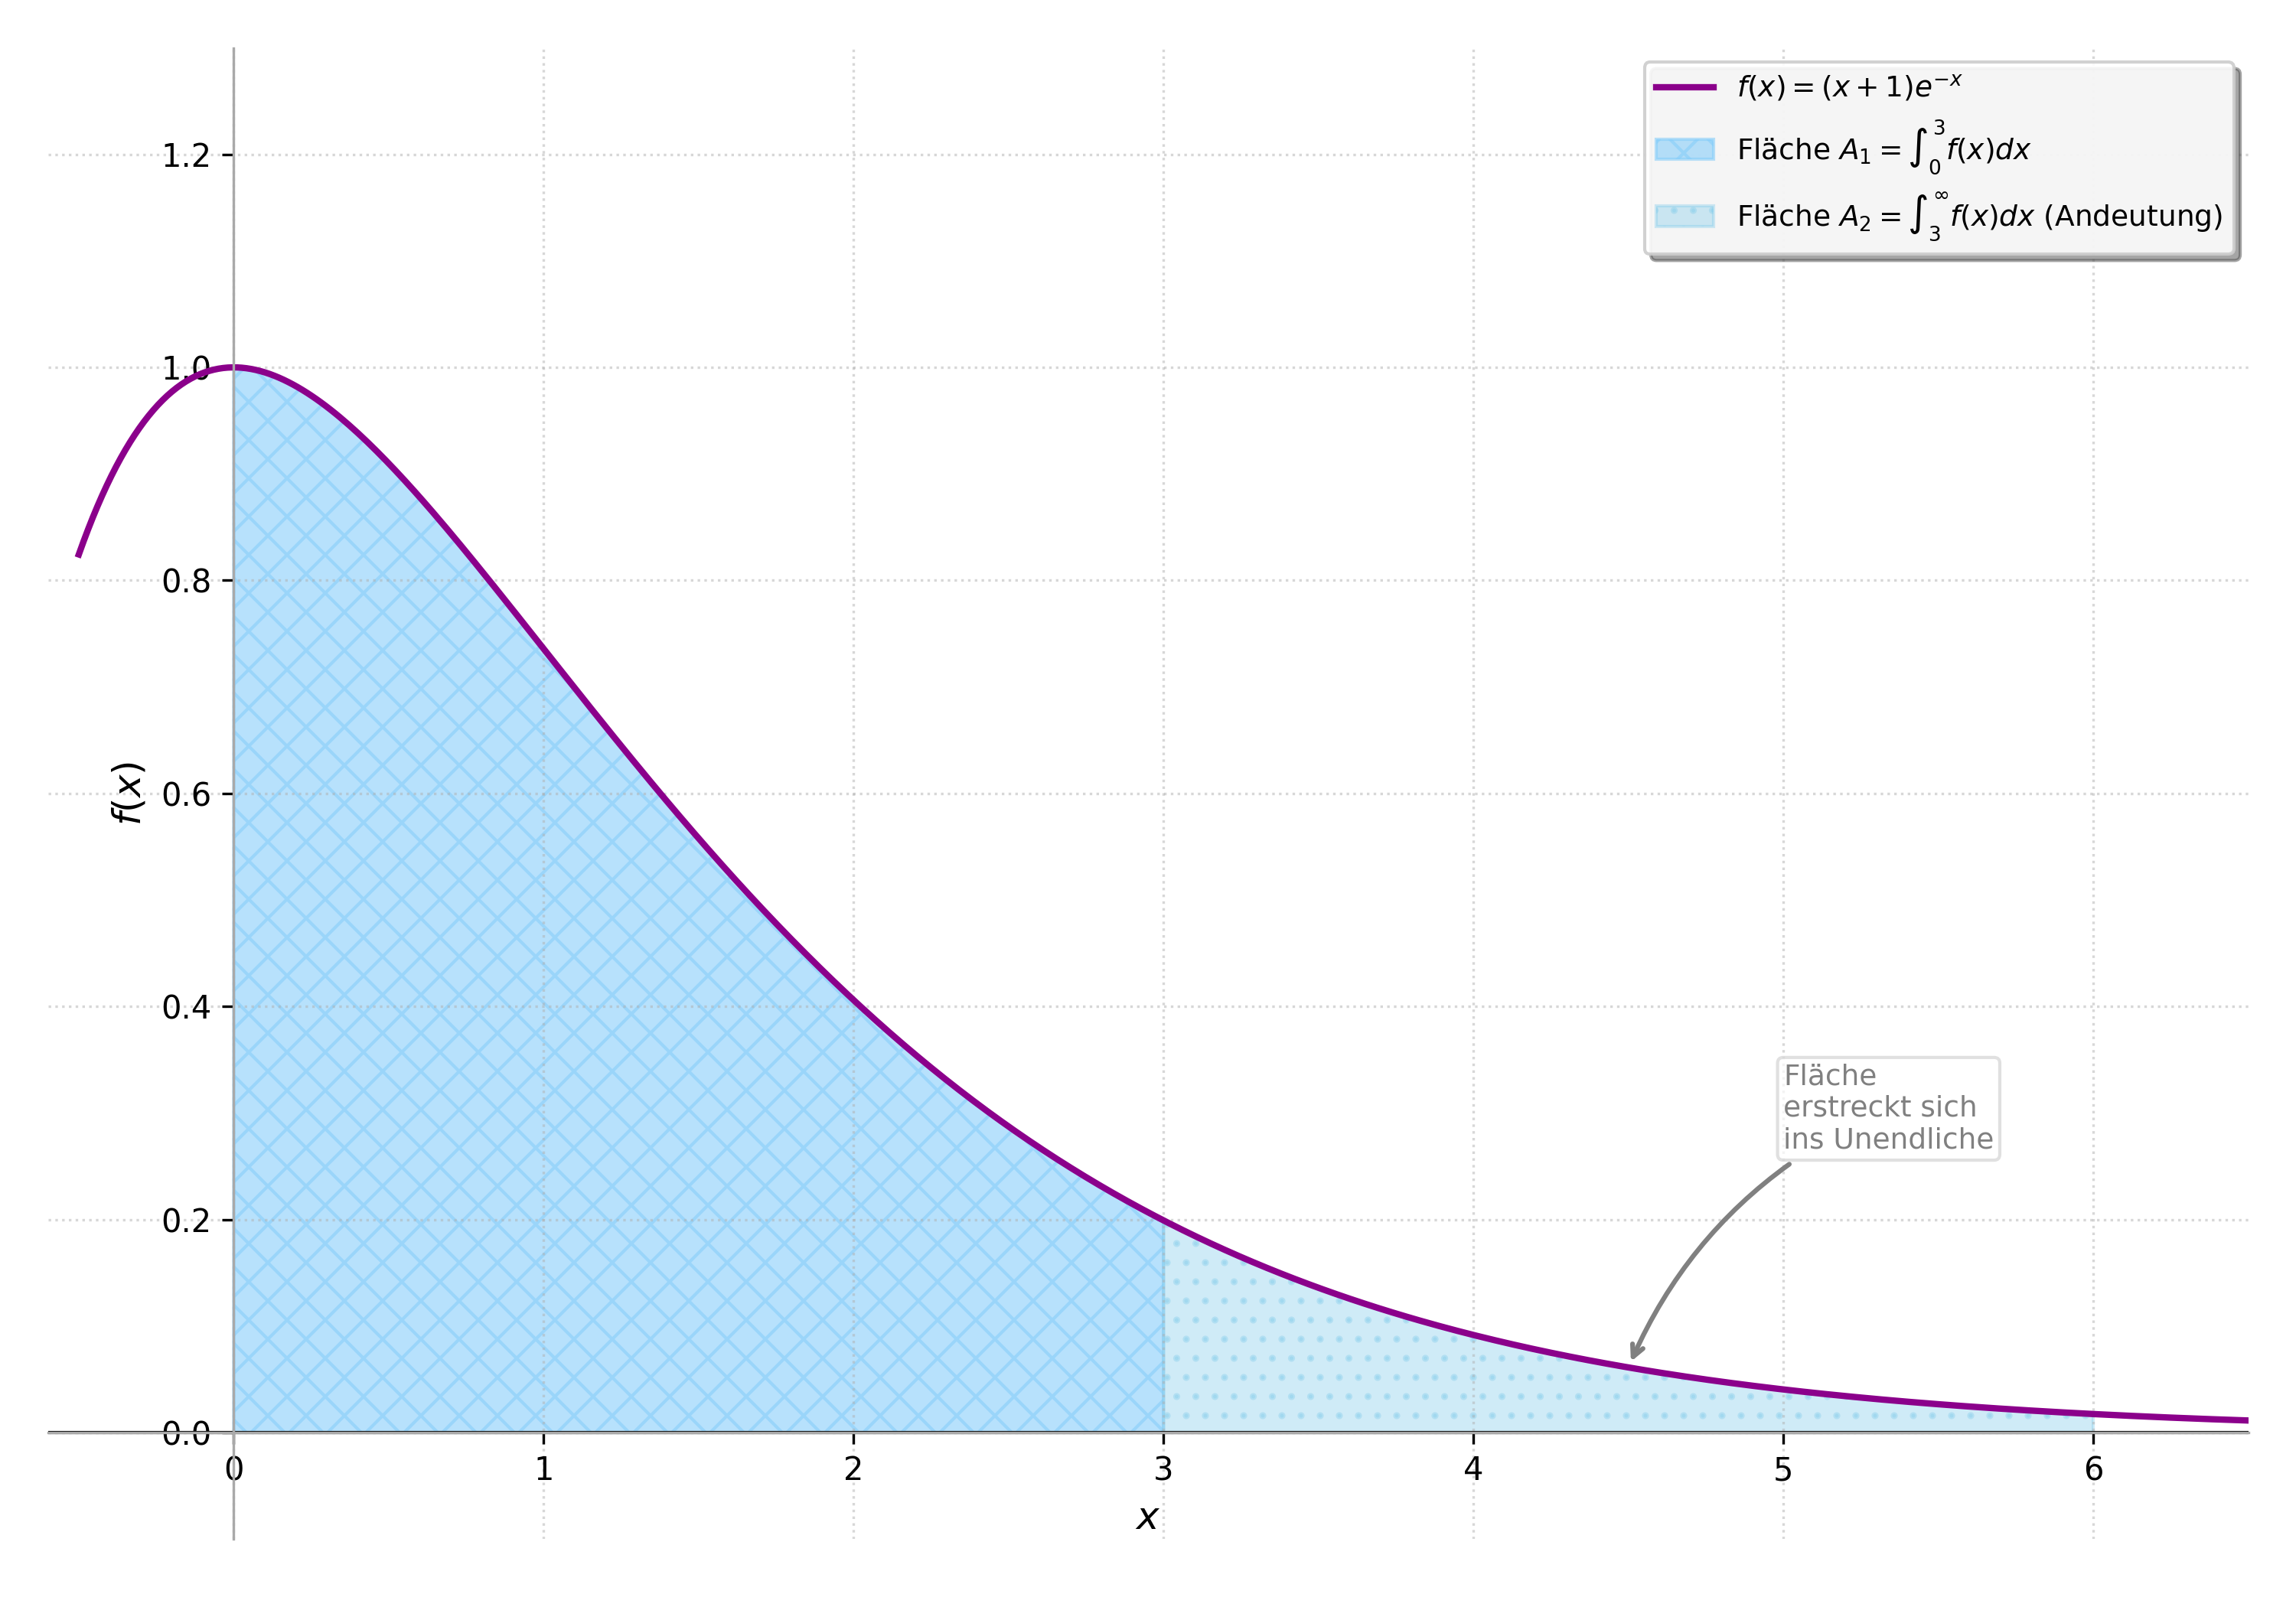
\includegraphics[width=0.8\textwidth]{grafiken/Integral_Flaeche_xplus1ehochminusx.png}
                \captionof{figure}{Fläche unter $f(x)=(x+1)e^{-x}$}
                \label{fig:flaeche_xplus1ehochminusx}
            \end{center}
            
    \item \textbf{Rekonstruktion einer Exponentialfunktion und Tangente:}
        Eine Funktion $f$ ist gegeben durch $f(x) = (ax+b)e^{-x}$. Der Graph von $f$ hat im Punkt $P(0|2)$ eine Tangente, die parallel zur Geraden $y=3x-5$ ist.
        \begin{itemize}
            \item Bestimme die Werte der Parameter $a$ und $b$.
            \begin{tippumgebung}{Bedingungen aufstellen}
            'Graph geht durch $P(0|2)$' $\implies f(0)=2$.
            'Tangente in $P(0|2)$ parallel zu $y=3x-5$' $\implies f'(0) = 3$.
            Bilde $f'(x)$ mit der Produkt- und Kettenregel.
            \end{tippumgebung}
            \item Bestimme die Gleichung der Tangente an den Graphen von $f$ im Punkt $P(0|2)$.
            \item Untersuche die Funktion $f(x)$ mit den gefundenen Parametern auf Nullstellen und Extrempunkte.
        \end{itemize}

    \item \textbf{Schar von Exponentialfunktionen (Schwer):}
        Gegeben ist die Funktionenschar $f_k(x) = x^2 e^{kx}$ mit dem Scharparameter $k \in \mathbb{R}$, $k \neq 0$.
        \begin{itemize}
            \item Bestimme die Nullstellen von $f_k(x)$.
            \item Bestimme die erste Ableitung $f_k'(x)$. Für welche Werte von $x$ (in Abhängigkeit von $k$) ist $f_k'(x)=0$?
            \item Untersuche die Art der Extremstellen in Abhängigkeit von $k$. (Tipp: Betrachte die Fälle $k>0$ und $k<0$ getrennt für das Verhalten der zweiten Ableitung oder den Vorzeichenwechsel der ersten Ableitung).
            \item Gibt es Werte für $k$, sodass die Funktion keine Extrempunkte besitzt?
        \end{itemize}
\end{enumerate}
\end{aufgabenumgebung}


\begin{kurzknappumgebung}{Exponentialfunktionen – Das Wichtigste im Überblick}
\begin{itemize}
    \item \textbf{Die natürliche Exponentialfunktion $f(x)=e^x$:}
        \begin{itemize}
            \item Basis $e \approx 2,71828\dots$ (Eulersche Zahl).
            \item Definitionsbereich $D_f = \mathbb{R}$, Wertebereich $W_f = (0, \infty)$.
            \item Keine Nullstellen, y-Achsenabschnitt bei $(0|1)$.
            \item Streng monoton steigend, linksgekrümmt.
            \item $\lim_{x \to -\infty} e^x = 0$ (horizontale Asymptote $y=0$), $\lim_{x \to \infty} e^x = \infty$.
            \item Besondere Eigenschaft: $(e^x)' = e^x$ und $\int e^x \,dx = e^x + C$.
        \end{itemize}
    \item \textbf{Transformierte Exponentialfunktion $f(x) = a \cdot e^{k(x-c)} + d$:}
        \begin{itemize}
            \item Parameter $a, k, c, d$ bewirken Streckung/Stauchung, Spiegelung, Verschiebung.
            \item Ableitung $(e^{kx})' = k \cdot e^{kx}$. Stammfunktion $\int e^{kx} \,dx = \frac{1}{k}e^{kx} + C$.
        \end{itemize}
    \item \textbf{Allgemeine Exponentialfunktion $f(x) = b^x$ ($b>0, b\neq 1$):}
        \begin{itemize}
            \item Umwandelbar zu $b^x = e^{x \ln(b)}$.
            \item Ableitung $(b^x)' = b^x \cdot \ln(b)$.
            \item Stammfunktion $\int b^x \,dx = \frac{1}{\ln(b)}b^x + C$.
        \end{itemize}
    \item \textbf{Anwendung der Ableitungsregeln:} Produkt-, Quotienten- und Kettenregel sind essentiell für Kombinationen von $e^x$ mit Polynomen oder anderen Funktionen (z.B. $f(x) = P(x) \cdot e^{g(x)}$).
    \item \textbf{Nullstellen von $P(x) \cdot e^{g(x)}$:} Da $e^{g(x)}$ immer positiv ist, hängen die Nullstellen nur von den Nullstellen des Faktors $P(x)$ ab.
    \item \textbf{Grenzwerte:} Die $e$-Funktion 'dominiert' oft Polynome im Unendlichen (z.B. $\lim_{x\to\infty} x^n e^{-kx} = 0$ für $k>0$).
    \item \textbf{Kurvendiskussion:} Folgt den bekannten Schritten, wobei die speziellen Eigenschaften von $e^x$ (keine Nullstellen, immer positiv, Grenzwertverhalten) und die Ableitungsregeln berücksichtigt werden.
    \item \textbf{Integrationstechniken mit $e^x$:}
        \begin{itemize}
            \item Partielle Integration für Produkte wie $\int x e^x \,dx$.
            \item Integration durch Substitution für verkettete Funktionen wie $\int 2x e^{x^2} \,dx$.
        \end{itemize}
    \item \textbf{Anwendungen:} Beschreibung von Wachstums- und Zerfallsprozessen, Flächenberechnungen, Mittelwerte, uneigentliche Integrale.
\end{itemize}
\end{kurzknappumgebung}

\begin{infoboxumgebung}{Ausblick: Logarithmusfunktionen – Die andere Seite der Medaille}
Mit den Exponentialfunktionen hast du eine unglaublich mächtige Funktionsklasse kennengelernt, die in unzähligen Bereichen der Wissenschaft und des Alltags Anwendung findet. Sie beschreiben Prozesse, bei denen sich etwas proportional zu seinem aktuellen Bestand ändert – das klassische Merkmal von Wachstum und Zerfall.

Doch was, wenn wir die umgekehrte Frage stellen? Wenn wir wissen, wie groß ein Bestand ist, und wissen wollen, wie viel Zeit vergangen ist? Oder wenn wir eine Gleichung wie $e^x = 100$ nach $x$ auflösen wollen? Hier kommt die \textbf{Logarithmusfunktion} ins Spiel, insbesondere der \textbf{natürliche Logarithmus ($\ln x$)}, der die direkte Umkehrfunktion zur natürlichen Exponentialfunktion $e^x$ ist.

Im nächsten Kapitel werden wir uns genau diese Logarithmusfunktionen ansehen:
\begin{itemize}
    \item Wie sind sie definiert und welche Eigenschaften haben sie?
    \item Wie sehen ihre Graphen aus (Tipp: Spiegelung von $e^x$ an $y=x$)?
    \item Wie leitet man Logarithmusfunktionen ab und wie bildet man ihre Stammfunktionen?
    \item Wie können wir sie in Kurvendiskussionen und Anwendungsaufgaben nutzen?
\end{itemize}
Du wirst sehen, dass Exponential- und Logarithmusfunktionen wie zwei Seiten derselben Medaille sind und zusammen ein unschlagbares Team bilden, um eine riesige Bandbreite an Problemen zu lösen. Die Werkzeuge der Differential- und Integralrechnung werden uns auch hier treue Dienste leisten.
\end{infoboxumgebung}


\begin{aufgabenumgebung}{Checkliste: Die Exponentialfunktion im Kern verstehen}
Die Exponentialfunktion ist in vielerlei Hinsicht besonders. Diese Fragen helfen dir, dein Verständnis zu vertiefen:

\begin{enumerate}[label=(\alph*)]
    \item \textbf{Die Eulersche Zahl $e$ und die natürliche Exponentialfunktion:}
    \begin{itemize}
        \item Warum wird $f(x)=e^x$ als die 'natürliche' Exponentialfunktion bezeichnet? Welche einzigartige Eigenschaft hat ihre Ableitung, und was bedeutet das für die Steigung ihres Graphen an jeder Stelle $x$?
        \item Vergleiche die Graphen von $y=2^x$, $y=e^x$ und $y=3^x$ in einer Skizze. Wo schneiden sie die y-Achse? Welche Funktion wächst für $x>0$ am schnellsten, welche am langsamsten? Wie verhält es sich mit ihren Steigungen an der Stelle $x=0$?
    \end{itemize}
    \item \textbf{Transformationen und Asymptoten:}
    Betrachte die Funktion $g(x) = A \cdot e^{k(x-B)} + C$.
    \begin{itemize}
        \item Erkläre, wie sich die Parameter $A, k, B, C$ jeweils auf den Graphen der Grundfunktion $y=e^x$ auswirken (Streckung, Stauchung, Spiegelung, Verschiebung).
        \item Welche Gleichung hat die waagerechte Asymptote von $g(x)$? Wie hängt diese vom Parameter $C$ ab? Warum kann der Graph diese Asymptote nie schneiden, wenn $A \neq 0$?
        \item Wenn $A>0$ und $k>0$: Ist die Funktion streng monoton steigend oder fallend? Was passiert, wenn $k<0$ ist?
    \end{itemize}
    \item \textbf{Von $b^x$ zu $e^{kx}$:}
    \begin{itemize}
        \item Erkläre mit eigenen Worten, warum jede Exponentialfunktion $f(x)=b^x$ (mit $b>0, b\neq1$) auch in der Form $f(x)=e^{kx}$ geschrieben werden kann. Welchen Wert hat $k$ in diesem Fall?
        \item Nutze diese Umschreibung, um die Ableitungsregel $(b^x)' = b^x \ln(b)$ aus der Regel $(e^{kx})' = k e^{kx}$ herzuleiten.
    \end{itemize}
    \item \textbf{Grenzwertverhalten und Dominanz:}
    \begin{itemize}
        \item Warum ist $\lim_{x \to -\infty} e^x = 0$, aber $\lim_{x \to \infty} e^x = \infty$?
        \item Betrachte eine Funktion $h(x) = x^n \cdot e^{-x}$ (mit $n \in \mathbb{N}$). Warum ist $\lim_{x \to \infty} h(x) = 0$, obwohl $x^n$ gegen $\infty$ geht? Welche Funktion 'dominiert' hier das Verhalten für große $x$?
    \end{itemize}
\end{enumerate}
\end{aufgabenumgebung}


\begin{aufgabenumgebung}{Checkliste: Exponentialfunktionen in der Analysis anwenden}
Die Analyse von Funktionen mit Exponentialtermen erfordert oft eine Kombination verschiedener Werkzeuge.

\begin{enumerate}[label=(\alph*)]
    \item \textbf{Nullstellen von $f(x) = P(x) \cdot e^{g(x)}$:}
    Wenn du die Nullstellen einer Funktion suchen sollest, die ein Produkt aus einem Polynom $P(x)$ und einem Exponentialterm $e^{g(x)}$ ist:
    \begin{itemize}
        \item Warum kannst du dich bei der Nullstellensuche ausschließlich auf den Faktor $P(x)$ konzentrieren?
        \item Gilt eine ähnliche Regel auch für die Nullstellensuche der Ableitung $f'(x)$ solcher Funktionen? (Tipp: Leite $P(x)e^{g(x)}$ allgemein mit Produkt- und Kettenregel ab und schaue, ob du $e^{g(x)}$ ausklammern kannst).
    \end{itemize}
    \item \textbf{Extremwertbestimmung bei $e$-Funktionen:}
    Betrachte die Funktion $f(x) = x^2 e^{-x}$.
    \begin{itemize}
        \item Welche Ableitungsregeln benötigst du, um $f'(x)$ und $f''(x)$ zu bilden?
        \item Wie gehst du vor, um die lokalen Extrempunkte zu finden? Erkläre die notwendige und die hinreichende Bedingung.
        \item Was erwartest du für das Verhalten von $f(x)$ für $x \to \infty$ und $x \to -\infty$? Wie hilft dir das, deine gefundenen Extrema einzuordnen (lokal vs. global)?
    \end{itemize}
    \item \textbf{Integrationstechniken im Kontext von $e$-Funktionen:}
    \begin{itemize}
        \item Für das Integral $\int (2x) e^{x^2} dx$: Welche Integrationstechnik bietet sich hier an und warum? Identifiziere die 'innere Funktion' und ihre Ableitung.
        \item Für das Integral $\int (x+1) e^x dx$: Welche Integrationstechnik ist hier typischerweise erfolgreich und warum? Wie würdest du die Faktoren für diese Technik wählen?
        \item Kannst du $\int e^{x^2} dx$ mit den in diesem Kapitel gelernten Methoden als elementare Funktion darstellen? (Tipp: Nicht jede Funktion hat eine einfach darstellbare Stammfunktion.)
    \end{itemize}
    \item \textbf{Interpretation im Anwendungskontext (Wachstum/Zerfall):}
    Ein Medikament wird im Körper exponentiell abgebaut, z.B. nach $M(t) = M_0 e^{-kt}$.
    \begin{itemize}
        \item Was bedeutet $M_0$ und was bedeutet ein größeres $k$ für den Abbauprozess?
        \item Die Ableitung $M'(t)$ gibt die momentane Abbaurate an. Ist $M'(t)$ positiv oder negativ? Warum ist das sinnvoll? Was passiert mit der Abbaurate für große $t$?
        \item Das bestimmte Integral $\int_{t_1}^{t_2} M(t) dt$ könnte als eine Art 'kumulierte Medikamentenbelastung' im Zeitintervall $[t_1, t_2]$ interpretiert werden. Welche Einheit hätte dieses Integral, wenn $M(t)$ in mg und $t$ in Stunden gemessen wird?
    \end{itemize}
\end{enumerate}
\end{aufgabenumgebung}

\begin{fehlerboxumgebung}{Interpretation von Grenzwerten und Asymptoten bei e-Funktionen}
Das Verhalten von Exponentialfunktionen im Unendlichen oder in Kombination mit Polynomen birgt einige Tücken:
\begin{itemize}
    \item \textbf{Asymptote bei $e^{kx}$ falsch bestimmt:} Die Funktion $f(x)=e^{kx}$ hat für $x \to -\infty$ die Asymptote $y=0$, wenn $k>0$ ist. Wenn aber $k<0$ (z.B. $f(x)=e^{-2x}$), dann gilt $\lim_{x \to \infty} e^{-2x} = 0$. Die Richtung, in der die x-Achse Asymptote ist, hängt vom Vorzeichen von $k$ ab! Bei $f(x)=A e^{k(x-B)} + C$ ist die Asymptote immer $y=C$.
    \item \textbf{Dominanz falsch eingeschätzt bei $P(x) \cdot e^{kx}$:} Für $x \to \infty$:
        \begin{itemize}
            \item Wenn $k>0$, 'gewinnt' der $e^{kx}$-Term gegen jedes Polynom $P(x)$, d.h. $P(x)e^{kx} \to \pm\infty$ (abhängig vom Vorzeichen von $P(x)$ für große $x$).
            \item Wenn $k<0$ (also $e^{-|k|x}$), 'gewinnt' der $e^{-|k|x}$-Term und geht schneller gegen 0, als $P(x)$ gegen $\infty$ geht. Also $P(x)e^{-|k|x} \to 0$.
        \end{itemize}
    Merke dir: Die Exponentialfunktion ist sehr 'stark' in ihrem Verhalten im Unendlichen.
    \item \textbf{Nullstellen von $P(x)e^{kx}$:} Die Nullstellen werden \textit{nur} durch $P(x)=0$ bestimmt, da $e^{kx}$ niemals Null wird. Manchmal wird fälschlicherweise versucht, $e^{kx}=0$ zu lösen.
\end{itemize}
Eine Skizze und die Betrachtung der Vorzeichen der beteiligten Faktoren helfen oft, Fehler zu vermeiden.
\end{fehlerboxumgebung}